\documentclass[upright, contnum]{umemoria}
\depto{DEPARTAMENTO DE CIENCIAS DE LA COMPUTACIÓN}
\author{CAMILO JOSÉ GÓMEZ NÚÑEZ}
\title{DISEÑO E IMPLEMENTACIÓN DE UN SISTEMA DE MENSAJERÍA ANÓNIMA BASADO EN DC-NET}
\auspicio{}
\date{MARZO 2017}
\guia{ALEJANDRO HEVIA ANGULO}
\carrera{MAGÍSTER EN CIENCIAS, MENCIÓN COMPUTACIÓN}
\memoria{TESIS PARA OPTAR AL GRADO DE}
\comision{\ }{\ }{\ }

\usepackage{lipsum}

\usepackage[utf8]{inputenc}
\usepackage[T1]{fontenc}
\usepackage[nottoc,numbib]{tocbibind}
\usepackage{pstricks}
\usepackage{cancel}

\newcommand{\nb}[3]{
		{\colorbox{#2}{\bfseries\sffamily\scriptsize\textcolor{white}{#1}}}
		{\textcolor{#2}{\sf\small$\blacktriangleright$\textit{#3}$\blacktriangleleft$}}}
		
\newcommand{\todo}[1]{\begin{center}\nb{ToDo}{red}{#1}\end{center}}
\newcommand{\todoline}[1]{\nb{ToDo}{red}{#1}}

\begin{document}

\frontmatter
\maketitle

\begin{abstract}
{\lipsum[1-4]}
\end{abstract}

\begin{dedicatoria} % opcional
Una dedicatoria corta. Por ejemplo, \emph{A los creadores de U-Campus}
\end{dedicatoria}

\begin{thanks} % opcional
\lipsum[1-2]
\end{thanks}
\cleardoublepage

\tableofcontents
% \listoftables % opcional
% \listoffigures % opcional

\mainmatter

\chapter{Introducción}\label{cap1}

\section{Anonimato en Internet}

Fruto tanto de las primeras revelaciones del grupo 
\emph{Wikileaks}\footnote{\url{https://wikileaks.org/}} en el año 2006, 
así como de la información revelada por el ex agente de la \emph{CIA}, 
\emph{Edward Snowden}\footnote{\url{http://www.huffingtonpost.com/news/nsa/}} 
en el año 2013, muchos usuarios han modificado su comportamiento de navegación 
por \emph{Internet} simplemente por el hecho de tener la presunción que todos 
sus movimientos están siendo registrados por organismos de Estado, a pesar de 
no ser amenaza a la seguridad de ninguna nación.

Por ende, usuarios de todo el mundo han comenzado a reclamar por su derecho a 
la privacidad\footnote{\url{http://www.livescience.com/37398-right-to-privacy.html}}, por ejemplo, tomando 
acciones que ocultan las páginas que visitan navegando en Internet de los 
organismos de Estado, o de cualquier tercero, que estén monitoreando y/o 
recopilando dichas visitas. Existe una basta comunidad compuesta por 
activistas de derechos humanos, abogados, ONGs, académicos y profesionales 
que abogan por que se haga valer el legítimo derecho a la 
privacidad de los usuarios de Internet, argumentando la importancia del 
anonimato\footnote{\url{https://www.derechosdigitales.org/anonimato/}} 
\footnote{\url{http://www.ted.com/talks/glenn_greenwald_why_privacy_matters}}, 
y motivando su tratamiento desde una perspectiva científica, brindando 
herramientas y protocolos que puedan asegurar el anonimato en Internet de 
manera segura, eficaz y eficiente. El trabajo de esta tesis está motivado por 
dicho objetivo.

Hoy en día navegar de manera anónima en Internet se realiza principalmente 
usando el software \emph{TOR}\footnote{\url{https://www.torproject.org/}}, 
el cual en su versión más popular consiste en un explorador web (variante de 
\emph{Firefox}\footnote{\url{https://www.mozilla.org/en-US/firefox}}) que 
ejecuta el protocolo \emph{onion-routing} (detallado en la siguiente sección), 
el cual permite dos objetivos: (1) ocultar la identidad del usuario tanto al 
proveedor del servicio que está consumiendo (página web que está visitando), 
como de algun observador externo, y (2) acceder a servicios ``ocultos'' que 
solo son accesibles por medio de \emph{TOR}. En este trabajo nos 
concentraremos en el primer objetivo solamente, detallando la manera en que 
\emph{TOR} logra ocultar la identidad del usuario del servicio. Es importante 
nombrar que \emph{TOR} no es la única manera de navegar de manera anónima en 
Internet: protocolos como \emph{mix-networks} y \emph{DC-Nets} (tema central 
en esta tesis) también logran ocultar la identidad del usuario.

El anonimato, más allá de su atractivo científico, es una problemática 
socialmente difícil de abordar. Esto se debe a que invoca prejuicios y dilemas 
éticos que, puestos en un contexto poco informado, pueden llegar a generar 
aprehensión e incluso rechazo. Parte de las aprehensiones se deben a la 
posibilidad de realizar acciones ilícitas bajo el paraguas del anonimato, lo 
cual puede impedir la persecucion policial de delitos donde el criminal use 
herramientas que permitan anonimato efectivo. Entre estas acciones se pueden 
mencionar: denuncias falsas, compra/venta de drogas, distribución de material 
pornográfico infantil, fraude, \emph{bullying}, etc. ¿Deberían los científicos 
crear y promover herramientas que permitan esas acciones? ¿Valen la pena las 
ventajas del anonimato como para permitir la realización de estas acciones sin 
la posibilidad de perseguir a sus ejecutores? Estas son algunas preguntas que 
todo científico debería realizarse antes de generar un trabajo (independiente 
del tema de investigación) que afecta directamente la sociedad en que está 
envuelto. Desde el punto de vista del autor, la labor del científico es 
siempre generar el ``mejor conocimiento'' posible, expandir la barrera del 
conocimiento humano, y al mismo tiempo, estar conciente de las posibles 
implicancias que posea en otras esferas de la sociedad, como por ejemplo en 
este caso, facilitar acciones ilícitas a través de Internet. Pese a los 
potenciales usos negativos, es nuestra opinion que los sistemas de anonimato 
pueden ser herramientas efectivas contra la censura y violacion de la 
privacidad existentes en regimenes autoritarios. También en situaciones de 
denuncia donde los potenciales enviadores arriesgan su vida (denuncias de 
narcotráfico o espionaje). El problema de limitar el uso socialmente negativo 
de estas tecnologias es un problema de investigacion abierto y extremadamente 
interesante.  

\section{Protocolos de Anonimato}

\subsection{\emph{Mix-networks}}

Una alternativa para anonimizar mensajes lo entregan protocolos de mezcla de 
mensajes, comúnmente llamados \emph{mixnets}. Una \emph{mixnet} consiste en un 
proceso iterativo donde un conjunto de mensajes encriptados es mezclado 
(permutado) en forma secuencial por una colección de servidores o 
``\emph{mix-servers}'' \cite{chaum1981untraceable}. Este proceso puede verse 
como una ``mezcla no invertible'' donde la \emph{mixnet} disocia datos 
referentes a la emisión del mensaje (identidad, tiempo del envío, etc.) con el 
mensaje mismo, impidiendo individualizar a un emisor con un mensaje en 
particular. El principal problema de este protocolo es que el anonimato se 
preserva gracias a la participación de \emph{mix-servers} honestos, y por ende 
requiere de una ``tercera parte confiable''. Para garantizar la privacidad de 
la mezcla (esto es, el anonimato), es que se utilizan varias etapas 
(servidores) de mezcla, pues basta que un servidor sea honesto, para que la 
permutación realmente permanezca oculta. Sin embargo, el depender de varios 
servidores de mezcla repercute en un proceso más ineficiente, resultando en 
una alta latencia al momento de enviar un mensaje. Importante es mencionar que 
la seguridad que, dado que utilizan típicamente encriptación de clave pública, 
se logra con una \emph{mixnet} es solamente computacional, esto es, 
eventualmente en un futuro donde sea posible adquirir un mayor poder de 
cómputo, el anonimato podría verse comprometido.

\subsection{\emph{Onion-Routing}}

El protocolo más utilizado hoy en día para proveer anonimato en la red es 
\emph{onion-routing} \cite{reed1998anonymous}, utilizado principalmente a 
través del software \emph{TOR}. Su popularidad viene dada principalmente por 
el carácter abierto que posee el proyecto. Esto le permite recibir 
contribuciones por parte de voluntarios todos los 
días\footnote{\url{https://www.torproject.org/getinvolved/volunteer.html.en}}, 
arreglando fallas que puedan existir, además de recibir permanentes análisis 
por parte de instituciones académicas que buscan la mejora, tanto del software 
como del protocolo subyacente. Si bien el sistema posee múltiples ventajas 
(llegando a ser recomendado por el mismo Snowden para ocultarse de las 
intromisiones de organismos de 
Estado\footnote{\url{https://www.inc.com/larry-kim/5-online-privacy-tips-from-edward-snowden.html}}), se sabe que 
varias falencias. Por ejemplo la vulnerabilidad descrita en 
\cite{syverson2001towards}, llegando incluso a poder romper el anonimato que 
éste provee si se posee la capacidad de monitorear toda la red (como la que 
poseen los distintos \emph{ISP} que proveen la conexión a Internet a los 
usuarios de la red). También es importante mencionar que el protocolo 
\emph{onion-routing} fue pensado bajo la amenaza de un adversario ``local'', 
es decir, uno que no puede monitorear toda la red. Este supuesto últimamente 
se ha ido debilitando, puesto que varias filtraciones muestran que, la 
\emph{NSA} en particular, efectivamente poseería la capacidad de monitorear 
todo Internet, haciendo inseguro al protocolo \emph{onion-routing}, y en 
consecuencia el software \emph{TOR}.

\section{La Cena de Criptógrafos}

David Chaum en el año 1985 propuso un protocolo que permitía el envío de 
mensajes de manera anónima entre un grupo de participantes 
\cite{Chaum:1985:SWI:4372.4373, chaum1988dining}. Dicho protocolo fue motivado 
con una historia llamada ``El Problema de la Cena de Criptógrafos'' 
(\emph{Dining Cryptographers Problem}), razón por la cual el protocolo desde 
entonces se conoce como \emph{DC-Net} (\emph{Dining Cryptographers Network}).

El problema es el siguiente: están tres criptógrafos cenando tranquilamente en 
su restorán favorito. Al terminar la cena, el mozo se acerca a su mesa y les 
comunica que su cena ya está pagada y que pueden irse a sus casas. Los 
criptógrafos, altamente consternados, se miran mutuamente y llegan a la 
conclusión de que debió haber sucedido una de dos cosas: (1) uno de ellos pagó 
la cuenta de manera anónima (haciéndose el amable e invitando al resto sin que 
ellos sepan), ó (2) la cuenta fue pagada por alguien distinto a ellos tres 
(como la \emph{NSA} por ejemplo), revelando la intromisión del organismo de 
inteligencia de EE.UU. en la vida de los criptógrafos. En esta situación, se 
hace necesario poder dilucidar este problema, pero sin comprometer (si es que 
fue el caso) al criptógrafo que pagó la cuenta de manera anónima. Por lo tanto 
los criptógrafos necesitan saber si uno de ellos pagó la cuenta (sin saber 
quién) o si fue alguien distinto.

David Chaum generaliza el problema de la siguiente manera: se tienen 3 
participantes (los criptógrafos) donde cada uno de ellos quiere comunicar un 
mensaje (pagó o no pagó la cena). El resultado del protocolo debe entregar, ya 
sea el mensaje de alguno de ellos (que pagó la cena), sin conocer el emisor de 
dicho mensaje, o bien que todos los mensajes fueron iguales (revelando que 
nadie pagó la cena, concluyendo que fue un agente externo). El protocolo debe 
poder mantener el anonimato del participante que envió el mensaje tanto para 
el resto de los participantes como para cualquier observador externo que esté 
monitoreando las conversaciones.

La solución propuesta supone el envío de solo un bit de información (si pagó o 
no pagó la cena). La solución generalizada consiste en los siguientes pasos:
\begin{enumerate}
    \item Cada par de participantes $(p_i, p_j)$ escogen un bit al azar 
    compartido $b_{ij}$. Además, se fija $b_{ij} = -b_{ji}$
    \item Cada participante $p_i$ calcula $b_i$ como el \texttt{XOR} binario 
    (denotado $\oplus$) entre todos los $b_{ij}$ que posee compartidos. Por 
    ejemplo, en el caso de la cena: $b_1 = b_{12} \oplus b_{13}$, $b_2 = b_{12}
     \oplus b_{23}$, $b_3 = b_{13} \oplus b_{23}$.
    \item Cada participante $p_i$ define su propio $M_i$, el cual 
    corresponderá al bit que quiere comunicar ($M_i = 1$ si pagó la cena, $0$ 
    si no).
    \item Cada $p_i$ revelará el valor $o_i = M_i \oplus b_i$.
    \item Cualquier $p_i$ u observador externo puede calcular el valor 
    $D = \displaystyle\bigoplus_i o_i$.
    \item Si $D = 1$, entonces uno de los participantes envió el mensaje 1 
    (alguien pagó la cena), si $D = 0$, todos los participantes enviaron el 
    mensaje 0 (la cena la pagó un agente externo a los participantes).
\end{enumerate}

\begin{figure}[H]
\centering
\begin{subfigure}[b]{0.4\textwidth}
    \begin{footnotesize}
\newcommand{\participK}[2]{
\begin{scope}[shift={(#1)}]
\draw [draw,fill=lightgray] (0pt,10pt) circle (5pt);
\draw [draw,fill=lightgray] (10pt,0pt) arc (0:180:10pt and 5pt);
\fill [lightgray] (-10pt,-10pt) rectangle (10pt,0pt);
\draw [draw] (10pt,0pt) -- (10pt,-10pt);
\draw [draw] (-10pt,0pt) -- (-10pt,-10pt);
\draw [draw] (5pt,-1pt) -- (5pt,-10pt);
\draw [draw] (-5pt,-1pt) -- (-5pt,-10pt);
\draw [anchor=center] (0pt,-2.5pt) node {#2};
\end{scope}
}
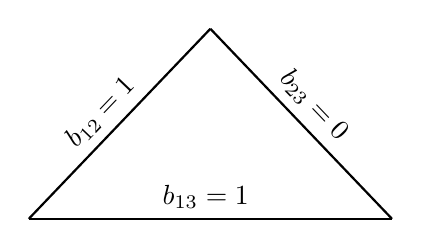
\begin{tikzpicture}
\begin{scope}
\path (18:6.9em) coordinate (P3);
\path (90:9em) coordinate (P2);
\path (162:6.9em) coordinate (P1);
\draw [thick] (P3) to node [anchor=south ,pos=0.5,swap,sloped] {$b_{23} = 0\ $} (P2);
\draw [thick] (P3) to node [anchor=south ,pos=0.5,swap,sloped] {$b_{13} = 1\ $} (P1);
\draw [thick] (P2) to node [anchor=south ,pos=0.5,swap,sloped] {$b_{12} = 1\ $} (P1);

\participK{P1}{$P_1$};
\participK{P2}{$P_2$};
\participK{P3}{$P_3$};
\end{scope}


\end{tikzpicture}
\end{footnotesize}
    \caption{Ilustración del bit al azar $b_{ij}$ compartido entre cada par de 
    participantes.}
    \label{2a}
\end{subfigure}
~
\begin{subfigure}[b]{0.4\textwidth}
    \begin{footnotesize}
\newcommand{\participK}[2]{
\begin{scope}[shift={(#1)}]
\draw [draw,fill=lightgray] (0pt,10pt) circle (5pt);
\draw [draw,fill=lightgray] (10pt,0pt) arc (0:180:10pt and 5pt);
\fill [lightgray] (-10pt,-10pt) rectangle (10pt,0pt);
\draw [draw] (10pt,0pt) -- (10pt,-10pt);
\draw [draw] (-10pt,0pt) -- (-10pt,-10pt);
\draw [draw] (5pt,-1pt) -- (5pt,-10pt);
\draw [draw] (-5pt,-1pt) -- (-5pt,-10pt);
\draw [anchor=center] (0pt,-2.5pt) node {#2};
\end{scope}
}
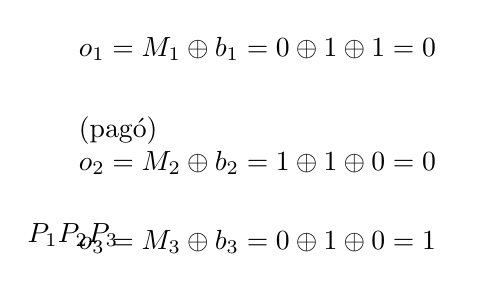
\begin{tikzpicture}

\begin{scope}
\path (0em,7em) coordinate (Q1);
\path (0em,3.5em) coordinate (Q2);
\path (0em,0em) coordinate (Q3);

\node [rectangle, right of=Q1, anchor=west, node distance=1.5em] {$o_1 = M_1 \oplus b_1 = 0 \oplus 1 \oplus 1 = 0$};
\node [rectangle, right of=Q2, anchor=west, node distance=1.5em, text width=136pt] {(pagó)\\$o_2= M_2 \oplus b_2 = 1 \oplus 1 \oplus 0 = 0$};
\node [rectangle, right of=Q3, anchor=west, node distance=1.5em] {$o_3= M_3 \oplus b_3 = 0 \oplus 1 \oplus 0 = 1$};

\participK{Q1}{$P_1$};
\participK{Q2}{$P_2$};
\participK{Q3}{$P_3$};
\end{scope}

\end{tikzpicture}
\end{footnotesize}

    \caption{Cálculo de $o_i$ por cada participante, dependiendo si pagó o no 
    la cena.}
    \label{2b}
\end{subfigure}

\protect\caption{Ejemplo de Cena de Criptógrafos donde uno de los 
participantes pagó la cena. En este caso $D = 0 \oplus 0 \oplus 1 = 1$. 
No es difícil observar que si ningún participante pagó la cena, $D = 0$.}
\label{fig:example_dcnet_chaum}
\end{figure}

Luego de proponer esta solución, David Chaum realiza el análisis de seguridad 
del protocolo (para detalles consultar el paper original 
\cite{chaum1988dining}), del cual concluye que el protocolo sugerido entrega 
anonimato de manera \emph{incondicional}: que incluso un adversario que posea 
todo el poder de cómputo posible no puede dar con una estrategia que le 
permita encontrar al emisor del mensaje con mejor probabilidad que $1/n$ 
(donde $n$ es la cantidad total de participantes).

Posteriormente se propone una manera de generalizar el protocolo para 
utilizarlo con mensajes más largos (de más de 1 bit), lo cual será 
visto en la siguiente sección.

\section{\emph{DC-Net} como protocolo de anonimato}

\emph{DC-Net} (\emph{Dining Cryptographers Network}) es un protocolo que 
permite enviar un mensaje de manera anónima a un grupo de participantes 
(llamado \emph{anonymity-set}). Este protocolo protege la identidad del emisor 
del mensaje de manera \emph{incondicional}, es decir, que ningún adversario 
(independiente del poder de cómputo que posea) puede encontrar a dicho emisor 
con una probabilidad mayor a $1/n$ (donde $n$ es el tamaño del 
\emph{anonymity set} o la cantidad total de participantes). Dicho adversario 
puede ser interno (uno de los participantes) o externo (por ejemplo, un 
observador externo que esté monitoreando todas las comunicaciones entre los 
distintos participantes).

A continuación se detallará la generalización del protocolo para permitir el 
envío de mensajes de largo arbitrario. Supongamos un \emph{anonymity set} de 
$n$ participantes $\{p_1, p_2, \ldots, p_n\}$. Sin pérdida de generalidad, 
supondremos que $p_1$ es el único participante que quiere enviar un mensaje 
(más adelante se discutirá el caso cuando dos o más participantes quieren 
enviar un mensaje). En este caso $M_1 = m \in 
\mathbb{Z}_q$\footnote{$\mathbb{Z}_q = \{1, 2, \ldots, q - 1\}$}, para todo el 
resto $M_i = 0$ $(\forall i \in \{2, \ldots, n\})$.

El primer paso, al igual que en el protocolo original, es generar valores (o 
claves) compartidos entre cada par de participantes. Cada par $\{p_i, p_j\}$ 
comparte un valor único $k_{ij}$ (y se define además que $k_{ij} = -k_{ji}$ y 
$k_{ii} = 0$).

\begin{figure}[H]
  \centering
    \includegraphics[width=0.5\textwidth]{imagenes/dcnet-general-03.png}
  \caption{Claves compartidas en DC-Net}
\end{figure}

Con esto, cada participante $p_i$ genera un valor igual a la suma de todas las 
claves compartidas que posee, esto es $K_i = \sum_{j=1}^n k_{ij}$. 
Luego, genera el valor $O_i = K_i + M_i$ que comunica al resto de los 
participantes. Este valor es la suma de la clave $K_i$ con el mensaje $M_i$, 
(recordemos que solo $p_1$ posee su mensaje distinto a 0, por lo que para el 
todo el resto de los participantes $O_i = K_i$). Finalmente, cada participante 
envia el valor $O_i$ al resto de los participantes (vía \emph{broadcast}, por 
ejemplo). Con esto, los valores $O_i$ quedan disponibles tanto para el resto 
de los participantes, como para cualquier observador externo.

Ahora solo queda encontrar el mensaje enviado por $p_1$. Para ello, se calcula 
el valor $D$ como la suma de todos los $O_i$ enviados por los participantes: 
$$D = \sum_{i=1}^n O_i \overset{(1)}{=} \sum_{i=1}^n K_i + \sum_{i=1}^n M_i 
\overset{(2)}{=} \sum_{i=1}^n K_i + m \overset{(3)}{=} m$$

La primera (1) igualdad se debe a la definición de $O_i$ y la separación de la 
suma en las dos componentes $K_i$ y $M_i$. La segunda (2) hace referencia al 
hecho que $M_i = 0$ $\forall i \geq 2$, por lo que solo ``sobrevive'' 
$M_1 = m$. Finalmente la tercera (3) se debe al hecho que las claves 
compartidas se cancelan mutuamente, debido a que $k_{ij} = -k_{ji}$. Por lo 
tanto, el valor $D$ corresponde al único mensaje enviado $m$, el cual es 
revelado al resto de los participantes, manteniendo en el anonimato a su 
emisor (en este caso, $p_1$).

Informalmente, el mensaje $m$ se oculta entre la suma de las claves 
compartidas. En principio conocer el valor de todas las claves compartidas (a 
menos que se coludan $n-1$ participantes), no es claro como poder dilucidar si 
un mensaje $m$ vino de un cierto valor $O_i$ revelado por participante $p_i$.

Ahora bien, el protocolo anteriormente descrito sufre de dos problemas: (1) el 
protocolo funciona sólo cuando un único participante envía un mensaje (de 
haber dos o más participantes con $M_i \neq 0$, se tendría que $D = \sum M_i$, 
por lo que sería imposible rescatar los mensajes individuales). Y, (2) no 
evita que participantes maliciosos envíen mensajes erróneos: por ejemplo, que 
participantes maliciosos envíen valores de claves compartidas distintos, 
causando que estas no se cancelen, evitando así la revelación del mensaje $m$ 
final. En este trabajo se detallará una variante que soluciona estos problema 
utilizando herramientas criptográficas que serán presentadas en el próximo 
capítulo.

\section{Objetivos del Trabajo}

\subsection{Objetivo General}

Diseñar e implementar una variante del protocolo \emph{DC-Net} que alcance 
mejores niveles de seguridad que los ofrecidos por otros protocolos 
actualmente utilizados para mantener anonimato. Además la variante debe estar 
optimizada para sistemas completamente distribuidos donde la implementación 
presente mejores resultados que las alternativas existentes, tomando en cuenta 
distintos factores como el tipo de seguridad alcanzada y la eficiencia en el 
envío de los mensajes.

\subsection{Objetivos Específicos}

\begin{itemize}
    \item Analizar las actuales soluciones (protocolos) que brindan anonimato 
    con el fin de evaluarlos críticamente y mejorarlos o contrastarlos con la 
    solución propuesta en el presente trabajo.
    \item Analizar otras implementaciones de variantes de \emph{DC-Net}, 
    identificando aspectos a mejorar, a fin de proponer una solución que 
    permita disminuir los supuestos de seguridad en que se basan dichas 
    soluciones.
    \item Testear la implementación realizada en distintos escenarios, 
    analizando el tiempo de ejecución en cada uno de ellos, con el objetivo 
    de encontrar el mejor contexto en que se desempeñaría la solución final.
    \item Crear un caso de prueba del sistema implementado, que sirva como 
    motivación a distintos posibles usos que se le pueda dar al código 
    realizado.
\end{itemize}

\section{Organización del Documento}

En el presente documento se describen los pasos que se siguieron para la 
propuesta de un diseño y una implementación de un sistema de mensajería que 
provee anonimato a los emisores basado en el protocolo \emph{DC-Net}. En el 
Capítulo \ref{cap2} se describen los antecedentes criptográficos 
necesarios para comprender la solución propesta, además de un análisis de 
soluciones similares propuestas en otros trabajos. Luego en el Capítulo 
\ref{cap3} se describe de manera detallada el diseño de la variante propuesta, 
especificando paso a paso lo que cada uno de los participantes debe realizar 
para poder contar con el sistema que se propuso como objetivo. Posteriormente 
en el Capítulo \ref{cap4} se presentan detalles de la implementación del 
diseño descrito anteriormente, incluido decisiones de diseño y cómo se fueron 
tomando para dar forma al sistema finalmente implementado. En este capítulo 
también se entrega una breve descripción de un caso de uso, una aplicación 
móvil. En el Capítulo \ref{cap5} se detallan los experimentos que se llevaron 
a cabo para testear la solución, incluyendo la evaluación de los tiempos de 
ejecución bajo distintos escenarios. Los resultados son discutidos en la parte 
final del capítulo. Luego en el Capítulo \ref{cap6} se brindan posibles 
mejoras tanto al protocolo diseñado como a la implementación realizada. 
Finalmente en el Capítulo \ref{cap7} se presentan tanto las conclusiones del 
presente trabajo, como las experiencias que dejaron tanto su diseño como su 
implementación.
\chapter{Antecedentes}
\section{\emph{Pedersen Commitments}}

Muchas primitivas criptográficas tienen como propósito ``ocultar'' información, es decir, transformar un cierto mensaje en una secuencia que, a primera vista, parecer ser totalmente aleatoria, y que solo puede ser ``comprendida'' (o transformada en el mensaje original) con el uso de una cierta clave secreta.

Existe una variante de la descripción anterior, que se presenta cuando la clave para descifrar un cierto texto secreto, es el mismo mensaje original. A un protocolo así se le llama \emph{protocolo de commitment} (compromiso), ya que no posee como finalidad comunicar un mensaje a otra persona de manera secreta, sino que más bien comprometer a un cierto participante a un cierto mensaje, dándole la oportunidad que este mensaje pueda permanecer en secreto, pero que \emph{a posteriori} la única manera de aceptar su mensaje es que revele el valor con el cual se comprometió en un principio.

\todo{Agregar descripción matemática de un protocolo de \emph{commitment}}

Existen varias herramientas matemáticas que nos permiten instanciar un protocolo de \emph{commitment}. En particular en este trabajo se utilizó el protocolo \emph{Pedersen Commitment}\cite{pedersen1991non}, el cual se basa en la dificultad de resolver el problema del logaritmo discreto \todoline{referencia para logaritmo discreto}.

\emph{Pedersen Commitment Scheme:} Sea $G_q$ un grupo de orden $q$, en donde el problema del logaritmo discreto se crea dificil de resolver. Sean $g,h$ generadores de $G_q$ elegidos de manera aleatoria. Sea $s \in \mathbb{Z}_q$ un secreto al cual el participante se comprometerá. Además sea $r \in \mathbb{Z}_q$ elegido aleatoriamente. Se le llama un \emph{Pedersen commitment} sobre $s$ al valor: $$c := g^s h^r$$

Los \emph{Pedersen commitments} brindan dos propiedades importantes: 
  ocultamiento perfecto (\emph{unconditionally hiding}) y 
  vinculación computacional (\emph{computationally binding}). 
Esto quiere decir que, si un participante calcula un \emph{commitment} sobre un 
  cierto valor $s$, 
  (1) la persona se compromete a dicho valor (pero sin revelarlo), ya que, 
  por un lado es imposible para un tercero conocer $s$ a partir de $c$, 
  y (2) es computacionalmente difícil demostrar que dentro de $c$ existe un valor distinto a $s$.

\section{\emph{Zero-Knowledge Proofs}}

Una \emph{zero-knowledge proof} permite a una persona poder demostrar el conocimiento de cierto valor $\alpha$ que cumple una propiedad 
  (en Inglés, \emph{statement}), sin revelar el valor 
  de $\alpha$ (el testigo) en esa demostración.
Se pueden construir demostraciones para diferentes tipos de propiedades 
  (\emph{statements}), como por ejemplo: el conocimiento de un logaritmo 
  discreto; la igualdad de diferentes logaritmos con distintas bases, además de combinaciones con operadores lógicos, entre otros. 
Además existen maneras para poder demostrar propiedades genéricas sobre
  logaritmos discretos 
  \cite{camenisch1997proof}.
  
  
Existe una estrecha relación entre \emph{commitment} y \emph{zero-knowledge proofs}, ya que estás últimas generalmente demuestran propiedades que poseen valores ``escondidos'' dentro de un \emph{commitment}, por lo que se puede convencer a un tercero que un cierto valor que no deseo revelar, sigue una cierta propiedad esperada.

\section{Implementaciones de \emph{DC-Nets} relacionadas}

El estudio de las DC-Nets como herramienta para brindar anonimato se ha incrementado en los últimos años, debido a los ataques encontrador a protocolos que ofrecían más rapidez a la hora de entregar mensajes, como lo es \emph{onion-routing}. En \cite{wright2002analysis} queda claro que el protocolo DC-Net es el que posee mayor seguridad a la hora de asegurar anonimato, pero sufre problemas de escalabilidad. Es por ello que los esfuerzos de muchas investigaciones ha sido como mantener la seguridad que ofrece el protocolo original, pero apuntando a arreglar los problemas de escabalidad que posee, y así construir una alternativa viable y eficiente a \emph{TOR} a la hora de mantenerse anónimo mientras se navega por Internet.

La primera implementación de una variante del protocolo DC-Net se encuentra en \cite{goel2003herbivore}, quienes presentan el sistema \emph{Herbivore}, el cual logra soslayar el problema de escalabilidad creando pequeños \emph{cluster} de participantes, reduciendo la cantidad de conexiones necesarias para enviar los mensajes anónimos. \todoline{encontrarle algo malo a herbivore y hablar sobre los tiempos y ancho de banda que alcanza}.

Luego de \emph{Herbivore} se deben mencionar los trabajos realizados por el grupo \emph{dedis (Decentralized and Distributed Systems Research)}\footnote{\url{http://dedis.cs.yale.edu/}} de \emph{Yale University}, quienes presentan tres sistemas: \emph{Dissent}, \emph{D3} y \emph{Verdict} \cite{corrigan2010dissent, wolinsky2012dissent, wolinsky2012scalable, corrigan2012proactively}. Estos sistemas tienen como principal objetivo atacar el problema de escalabilidad presente en las DC-Net. Esto lo logran utilizando servidores adicionales que participan en la comunicación entre los participantes, de esta manera los participantes no se deben conectar entre ellos (como una DC-Net tradicional), sino que se conectan a servidores intermediarios quienes funcionan como \emph{brokers} y entregan los mensajes a todos los participantes presentes. Los sistemas propuestos fueron evolucionando, llegando a realizarse pruebas con hasta 1000 participantes enviando mensajes. \todoline{encontrarle algo malo a dissent y amigos y hablar sobre los tiempos y ancho de banda que alcanza}.

\todo{Vuvuzela}

\todo{Riposte}

\todo{Riffle}
\chapter{Diseño de la variante \emph{DC-Net}}\label{cap3}

\section{Glosario de Términos}

\begin{itemize}
    \item Participante: agente que participa activamente del protocolo, ya sea 
    enviando un mensaje o contribuyendo para aumentar el tamaño del 
    \emph{anonimity-set} y así ocultar ``de mejor manera'' a los emisores de 
    mensajes. 
    \item Ronda: serie de pasos (descritos a partir de la próxima sección) que 
    se llevan a cabo (principalmente intercambiando mensajes entre los 
    participantes) con el objetivo de ir reduciendo, ronda a ronda, los mensajes 
    enviados por cada participante.  
    \item Mensaje: información que cada participante desea transmitir de 
    manera anónima. Generalmente se relacionará a un conjunto de caracteres 
    (representados como \emph{String}), en un cierto idioma, que se desea 
    comunicar.
    \item Sesión: conjunto de rondas que se necesitan realizar para que pueda 
    ser transmitido, a lo más, un mensaje por participante. Al principio de 
    cada sesión se le brinda la oportunidad a cada participante de decidir si 
    enviará o no un mensaje. Luego que cada participante realizó su decisión, 
    se inicia el protocolo descrito a continuación, que tiene como objetivo 
    que cada uno de los mensajes que se decidieron enviar, se envíen de manera 
    anónima al resto de los participantes.
    \item Sala: conjunto de participantes corriendo una sesión del protocolo.
    \item Observador Externo: cualquier agente (a excepción de los propios 
    participantes) que pueda estar monitoreando, tanto los mensajes 
    resultantes del protocolo, como mensajes intermedios intercambiados entre 
    los distintos participantes durante la realización del protocolo. A no ser 
    que se explicite, todos los mensajes del protocolo pueden ser monitoreados 
    por un observador externo y se consideran públicos.
    \item Adversario: agente que tiene como finalidad, ya sea encontrar al 
    emisor de un cierto mensaje, o bien, alterar el comportamiento ``normal'' 
    del protocolo (retrasándolo o impidiendo su total realización). Este 
    adversario puede ser un mismo participante del protocolo (al cual 
    llamaremos participante malicioso) o un observador externo.
    \item Canal de comunicación: enlace existente entre dos nodos del 
    sistema. Estos canales deben ser autenticados y no encriptados, es decir, todos los mensajes 
    enviados en el protocolos deben ir firmados utilizando un protocolo 
    de clave pública y éstos pueden enviarse ``en plano'', de manera que cualquier 
    monitoreo tiene la capacidad de observar los mensajes enviados, pero no 
    incorporar mensajes al sistema por parte de emisores no participantes del 
    protocolo.
\end{itemize}

\section{Diseño a primera vista}

El protocolo propuesto tiene como principal característica el no evitar las 
posibles colisiones que puedan producirse (idea que se distancia de otros protocolos 
que se enfocan en evitar la colisión de mensajes). De producirse la colisión, se 
debe resolver corriendo nuevas rondas del protocolo, pero solamente permitiendo 
que un subconjunto de los mensajes colisionados puedan re-enviarse en cada una 
de las rondas subsecuentes, produciendo así que en cada nueva ronda que se 
desarrolle, exista un menor número de mensajes colisionando, resultando así 
en rondas que se desarrollen sin colisión, enviándose los mensajes de manera 
solitaria, lo que les permite ser legibles por el resto de los participantes.

Las rondas que se desarrollan durante el protocolo son de dos tipos: reales y virtuales. 
En las rondas reales es necesario el envío de múltiples mensajes por parte de los participantes, 
involucrando el uso de varias herramientas criptográficas con el objetivo 
de evitar que participantes maliciosos alteren el normal desarrollo del protocolo. En cambio 
las rondas virtuales son tales que su resultado puede inferirse por rondas 
reales ejecutadas anteriormente, por lo que no es necesario el envío de 
ningún mensaje por parte de los participantes (las rondas reales cuestan trabajo por 
parte de los participantes, y las rondas virtuales no). Si la primera colisión 
de mensajes es de $n$ mensajes, eso implica que es necesario ejecutar $n$ rondas 
reales para poder resolver dicha colisión. 

% \begin{figure}
% \begin{centering}
% \footnotesize
% \pgfdeclarelayer{background layer}
% \pgfdeclarelayer{foreground layer}
% \pgfsetlayers{background layer,main,foreground layer}
% \begin{tikzpicture}[yscale=0.8]
% \begin{scope}[level distance=2.0cm,
% sibling distance=4cm,level/.style={sibling distance=3.8cm/#1},
% edge from parent/.style={draw,very thick},
% block/.style ={rectangle, draw=black, thick, text centered,  inner sep=0.12cm,font=\footnotesize},
% blockx/.style ={rectangle, dashed, draw=black, very thick, text centered,  inner sep=0.12cm,font=\footnotesize}]
% \begin{pgfonlayer}{foreground layer}
% \node[block] (n1){$\underbrace{M_1+M_2+M_3+M_4+M_5}_{\displaystyle (5,130)}$}
% %[edge from parent fork down]
% child {node (n21)[block] {$\underbrace{M_2+M_4}_{\displaystyle (2,28)}$} 
% child {node (n2x)[block,yshift=-1.6cm] {$\underbrace{M_2}_{\displaystyle (1,11)}$} edge from parent node[fill=white,anchor=east,xshift=-0.05cm] {$<14 $}}
% child {node (n2a)[blockx,yshift=-3.2cm] {$\underbrace{M_4}_{\displaystyle (1,17)}$}}
% edge from parent node[fill=white,anchor=east,xshift=-0.25cm] {$<26$}}
% child {node (n22)[blockx,yshift=-1.6cm] {$\underbrace{M_1+M_3+M_5}_{\displaystyle (3,102)}$}
% child {node (n31)[block,yshift=-3.2cm] {$\underbrace{M_3}_{\displaystyle (1,28)}$}edge from parent node[fill=white,anchor=east,xshift=-0.05cm] {$<34 $~}}
% child {node (n32)[blockx,yshift=-4.8cm] {$\underbrace{M_1+M_5}_{\displaystyle (2,74)}$}
% child {node (n3f)[block] {$\underbrace{M_1}_{\displaystyle (1,36)}$}edge from parent node[fill=white,anchor=east,xshift=-0.1cm] {$<37 $~}}
% child {node (n3g)[blockx,yshift=-1.6cm] {$\underbrace{M_5}_{\displaystyle (1,38)}$}}}
% };
% \end{pgfonlayer}

% %\node[anchor=east] at (n1.west){400 $\sim$};
% %\node[anchor=east] at (n21.west){410 $\sim$};
% %\node[anchor=west] at (n22.east){$\sim$ 420};

% %\draw (n1.north) node [anchor=south] {1};
% %\draw (n21.north) node [anchor=south] {2};
% %\draw (n2x.north) node [anchor=south] {3};

% \path []($(n1)+ (-5.0cm,1.0cm)$) -- node[above]{$C^{(k)}$} +(10cm,0);

% \begin{pgfonlayer}{background layer}
% \draw [densely dotted]($(n1)+ (-5.0cm,1cm)$) node [above,xshift=0.8cm]{round id $k$}-- +(12.1cm,0);
% \draw [densely dotted]($(n1)+ (-5.0cm,-1cm)$) node [above,xshift=0.8cm]{$1$}-- +(12.1cm,0) node[above,anchor=south west,xshift=-2.5cm]{$C^{(1)}=\sum^n_{i=1}O^{(k)}_1$};
% \draw [densely dotted]($(n1)+ (-5.0cm,-3cm)$) node [above,xshift=0.8cm]{$2$}-- +(12.1cm,0) node[above,anchor=south west,xshift=-2.5cm]{$C^{(2)}=\sum^n_{i=1}O^{(k)}_2$};
% \draw [densely dotted]($(n1)+ (-5.0cm,-5cm)$) node [above,xshift=0.8cm]{$3$}-- +(12.1cm,0) node[above,anchor=south west,xshift=-2.5cm]{$C^{(3)}=C^{(1)}-C^{(2)}$};
% \draw [densely dotted]($(n1)+ (-5.0cm,-7cm)$) node [above,xshift=0.8cm]{$4$}-- +(12.1cm,0) node[above,anchor=south west,xshift=-2.5cm]{$C^{(4)}=\sum^n_{i=1}O^{(k)}_4$};
% \draw [densely dotted]($(n1)+ (-5.0cm,-9cm)$) node [above,xshift=0.8cm]{$5$}-- +(12.1cm,0) node[above,anchor=south west,xshift=-2.5cm]{$C^{(5)}=C^{(2)}-C^{(4)}$};
% \draw [densely dotted]($(n1)+ (-5.0cm,-11cm)$) node [above,xshift=0.8cm]{$6$}-- +(12.1cm,0) node[above,anchor=south west,xshift=-2.5cm]{$C^{(6)}=\sum^n_{i=1}O^{(k)}_6$};
% \draw [densely dotted]($(n1)+ (-5.0cm,-13cm)$) node [above,xshift=0.8cm]{$7$}-- +(12.1cm,0) node[above,anchor=south west,xshift=-2.5cm]{$C^{(7)}=C^{(3)}-C^{(6)}$};
% \draw [densely dotted]($(n1)+ (-5.0cm,-15cm)$) node [above,xshift=0.8cm]{$14$}-- +(12.1cm,0) node[above,anchor=south west,xshift=-2.5cm]{$C^{(14)}=\sum^n_{i=1}O^{(k)}_{14}$};
% \draw [densely dotted]($(n1)+ (-5.0cm,-17cm)$) node [above,xshift=0.8cm]{$15$}-- +(12.1cm,0) node[above,anchor=south west,xshift=-2.5cm]{$C^{(15)}=C^{(7)}-C^{(14)}$};
% \end{pgfonlayer}

% \node[inner sep=0cm,fit=(n1) (n3g) (n2x)] (la) {};
% %\node at (la.south)[below=0.3cm,inner sep=0,font=\small] {(a) Collision resolution tree.};
% \end{scope}


% \end{tikzpicture}
% \par\end{centering}

% \protect\caption{Exemplary binary collision resolution tree with superposed receiving.
% In rounds 1,2,4,6 and 14, ciphertexts $O^{(k)}$ are transmitted,
% and $C^{(k)}$ is computed using these ciphertexts. In rounds 3,5,7
% and 15, no data is transmitted and $C^{(k)}$ is computed using data
% from the parent and the sibling node.}
% \label{supreceiving_tree-1}
% \end{figure}

\section{Compartición de Llaves}

Una ronda real comienza con el proceso de compartición de llaves entre cada 
par de participantes presentes en la sala. Este proceso debe realizarse, 
tomando un cuenta un posible adversario que esté monitoreando el canal de 
comunicación existente entre dos participantes cualquiera.

Para solucionar este problema se propone el uso del algoritmo 
\emph{Diffie-Hellman} \cite{diffie1976new}, el cual permite generar un valor 
secreto compartido entre dos agentes, cuyo canal de comunicación es 
monitoreado por un adversario.

Luego que cada par de participantes $\{P_i, P_j\}$ ejecuten el algoritmo 
\emph{Diffie-Hellman}, obtendrán un valor secreto $k_{ij}$ (se define que $k_{ij} = -k_{ji}$). 
Para futuros pasos 
del protocolo, es necesario que ejecuten este proceso dos veces, ya que es 
necesario que cuenten con un segundo valor compartido $r^k_{ij}$ (también se define 
que $r^k_{ij} = -r^k_{ji}$).

\subsection{\emph{Commitments} sobre las llaves}

Posteriormente cada participante $P_i$ debe realizar un \emph{commitment} a 
cada valor $k_{ij}$ que posee compartido con cada otro participante $P_j$, 
utilizando como aleatoriedad el segundo valor compartido $r^k_{ij}$. Esto 
resulta en que cada participante $P_i$ posee $n - 1$ de los siguientes valores 
$c_{k_{ij}} = g^{k_{ij}} h^{r^k_{ij}}$.

Luego de esto, cada participante $P_i$ generará dos valores, el primero será 
la suma de todas las llaves compartidas que posee $K_i = \sum k_{ij}$. El 
segundo valor será un \emph{commitment} sobre dicho valor, calculado utilizando 
los valores $c_{k_{ij}}$, esto es, 
$c_{K_i} = \prod c_{k_{ij}}$.

Finalmente cada participante $P_i$ enviará al resto de la sala vía 
\emph{broadcast} su \emph{commitment} $c_{K_i}$ junto con una 
\emph{zero-knowledge proof} demostrando que conoce los valores ``escondidos'' 
dentro del \emph{commitment}.

\subsection{Verificación de los valores enviados}

Cada participante, al recibir los \emph{commitments} enviados por el resto de la 
sala, debe verificar que se cumple la siguiente propiedad: $\prod c_{K_i} = 1$ 
(esto se debe a la cancelación que se debe producir al sumar las llaves). Si es que 
lo anterior no se produce, es resultado de que uno (o varios) de los participantes envió un 
valor incorrecto dentro de su \emph{commitment} respectivo, lo que implicaría una 
no cancelación de las llaves en etapas subsecuentes del protocolo, alterando la entrega 
de los mensajes.

Es posible encontrar al(a los) participante(s) culpable(s) de enviar información errónea. 
Para ello cada participante $P_j$ revelará cada valor $c_{k_{ji}}$ calculado anteriormente. 
Luego de esto, el resto de la sala puede verificar que se deben cumplir dos propiedades: 
(1) $c_{K_j} = \prod c_{k_{ji}}$, que se debe tener por definición, y 
(2) $c_{k_{ij}} c_{k_{ji}} = 1$, lo cual se debe a la cancelación de las llaves. Si alguna 
de las dos propiedades anteriores no se cumplen, el participante $P_j$ es malicioso y deben 
tomarse las medidas pertinentes que considere la sala.

\section{Formato del Mensaje}

Al principio de una sesión, cada participante $P_i$ debe decidir si desea comunicar 
un mensaje $msg$ al resto de la sala o no. De querer enviar un mensaje, habrán 
rondas que deberá enviar $m_i = msg$, y otras que enviará $m_i = 0$. De no querer 
transmitir un mensaje, en todas las rondas enviará $m_i = 0$. 

Para que el protocolo funcione correctamente, es necesario que dicho mensaje $m_i$ 
se concatene con otros valores, permitiendo el correcto manejo de colisiones de 
mensajes (es explicado más adelante en el documento). Estos valores auxiliares son 
los siguientes:
\begin{itemize}
    \item $b_i$: bit que indica si el participante está, en la presente ronda, 
    enviando un mensaje distinto a cero o no ($b_i = 1 \iff m_i \neq 0$).
    \item $pad_i$: cadena de bits aleatoria que se añade para prevenir colisión 
    de mensajes iguales, que podría desembocar en que la sesión nunca finalice.
\end{itemize}

Con estos valores establecidos, en cada ronda cada participante $P_i$ debe formar 
el siguiente valor $M_i$, mostrando en la Figura \ref{fig:M_sending} el formato cuando 
el participante envía $m_i \neq 0$, y en la Figura \ref{fig:M_not_sending} el formato 
cuando el participante envía $m_i = 0$ (que significa $M_i = 0$):

\begin{figure}[H]
  \centering
    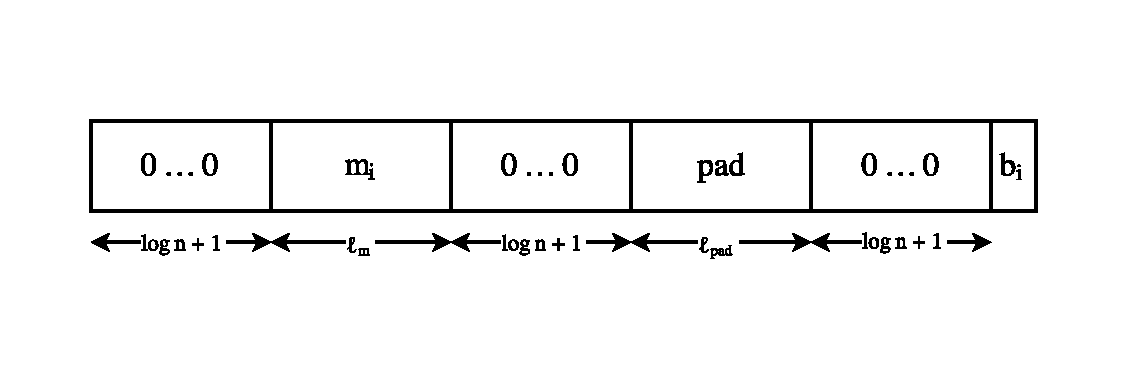
\includegraphics[width=1\textwidth]{imagenes/message-format(1).pdf}
  \caption{$M_i$ cuando se envía un mensaje}
  \label{fig:M_sending}
\end{figure}

\begin{figure}[H]
  \centering
    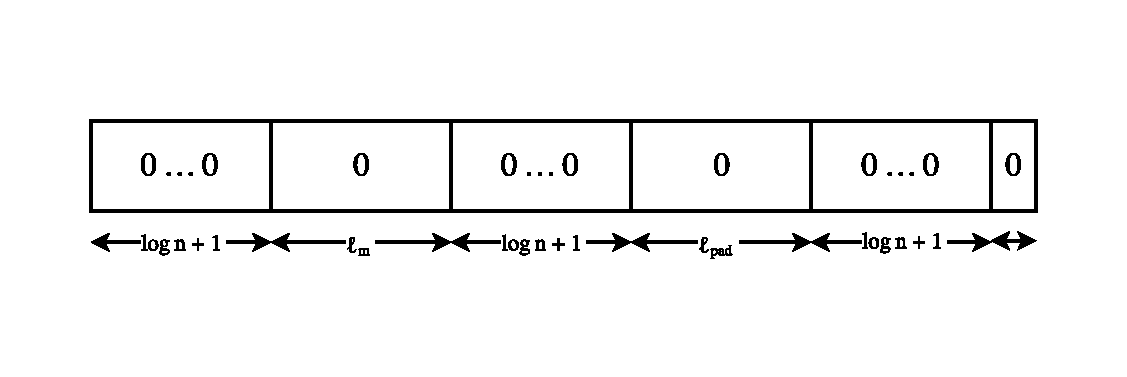
\includegraphics[width=1\textwidth]{imagenes/message-format-nomessage.pdf}
  \caption{$M_i$ cuando no se envía un mensaje}
  \label{fig:M_not_sending}
\end{figure}

Las cadenas de bits de solamente 0s puestas entre medio de los valores, sirven para 
prevenir \emph{overflows} de los valores, impidiendo que se altere el resultado 
final.

\section{Correctitud del Formato del Mensaje}

Para que el protocolo tenga un correcto funcionamiento en el manejo de colisiones, 
es imperioso que el formato del mensaje $M_i$ se respete por todos los participantes. 
Para ello se debe satisfacer una de las siguientes restricciones:
\begin{itemize}
    \item Si $b_i = 0$, entonces $m_i = 0$
    \item $b_i = 1$
\end{itemize}

En la primera alternativa, se le fuerza al participante a que si esta diciendo que 
no envía un mensaje ($b_i = 0$), no lo envíe ($m_i = 0$). En la segunda opción, se 
le permite cualquier valor de $m_i$ siempre y cuando se cumpla que $b_i = 1$.

\subsection{\emph{Commitments} sobre los valores individuales}

Para poder demostrar que el mensaje $M_i$ posee un correcto formato, cada participante $P_i$  
debe primero realizar \emph{commitments} a cada uno de los valores $\{m_i, pad_i, b_i\}$. 
Para ello, se escogen valores aleatorios $\{r_i^m, r_i^{pad}, r_i^b\}$ y se calculan 
los valores $c_{m_i} = g^{m_i} h^{r_i^m}; c_{pad_i} = g^{pad_i} h^{r_i^{pad}}; c_{b_i} = g^{b_i} h^{r_i^b}$ 
(\emph{commitments} a los valores individuales anteriormente descritos).

\subsection{\emph{Zero-knowledge Proof} sobre formato del mensaje}

Ahora es momento que cada participante genere una \emph{zero-knowledge proof} que 
demuestre que el mensaje $M_i$ esta bien formado. Para ello es necesario establecer 
primero si en la presente ronda el participante enviará un mensaje ($m_i \neq 0$) o 
no ($m_i = 0$).

\begin{enumerate}
    \item No envío de mensaje ($m_i = 0$): para demostrar que el formato es correcto 
    cuando no necesito enviar un mensaje, cada participante debe demostrar la primera 
    restricción que se mostró anteriormente, esto es, que $b_i = 0 \land m_i = 0$.
    
    Es importante notar que cuando sucede lo anterior, los valores de los 
    \emph{commitments} anteriormente descritos quedan de la siguiente manera: 
    $c_{m_i} = h^{r_i^m}; c_{b_i} = h^{r_i^b}$.
    
    Finalmente lo que el participante debe demostrar es que conoce los valores 
    $\{r_i^m, r_i^b\}$ contenidos en dichos \emph{commitments}.
    \item Envío de mensaje ($m_i \neq 0$): para demostrar que el formato es 
    correcto cuando necesito enviar un mensaje, debo demostrar la segunda 
    restricción, esto es solamente que $b_i = 1$.
    
    Al igual que en el caso anterior el \emph{commitment} relacionado queda con 
    un formato particular $c_{b_i} = g h^{r_i^b}$.
    
    En este caso se le va a pedir al participante demostrar que conoce $r_i^b$ 
    en $g^{-1} c_{b_i} = h^{r_i^b}$.
\end{enumerate}

Como no se puede saber si el participante enviará o no un mensaje 
(comprometería su anonimato) se va a solicitar que demuestre cualquiera de las 
dos condiciones anteriores. La \emph{zero-knowledge proof} que necesita demostrar 
cada participante es la siguiente: 
$$\mathtt{PoK_i^{format}} = PoK\{(r_i^m, r_i^b) : (c_{m_i} = h^{r_i^m} \land c_{b_i} = h^{r_i^b}) \lor (g^{-1} c_{b_i} = h^{r_i^b})\}$$

\subsection{Envío de valores a la sala}

Después de todos los cálculos anteriores, cada participante $P_i$ debe enviar 
al resto de la sala vía \emph{broadcast} los siguientes valores: 
$\{c_{m_i}, c_{pad_i}, c_{b_i}, \mathtt{PoK_i^{format}}\}$ (los tres \emph{commitments} 
calculados y la demostración correspondiente).

\subsection{Verificación de la demostración}

Después de que toda la sala haya recibido todos los conjuntos de valores enviados 
por cada uno de los participantes, es necesario verificar que la demostración sea 
correcta, y para ello solamente es necesario los valores de los \emph{commitments} 
acompañando la \emph{zero-knowledge proof}.

\section{Demostración de conocimiento del mensaje}

Cada particiante $P_i$ debe enviar un \emph{commitment} sobre el mensaje $M_i$ 
construido anteriormente, con el objetivo que más adelante envíe el mensaje que 
ha estado construyendo durante la presente ronda. Para construir dicho \emph{commitment} 
utilizará los \emph{commitments} de los valores individuales enviados anteriormente. 
Para ello calculará 
$c_{M_i} = f(c_{m_i}, c_{pad_i}, c_{b_i})$\footnote{$f(x, y, z) = x^{2^{|pad|}(n+1)} y^{(n+1)} z$} 
$= g^{M_i} h^{r_i^{M}}$ (donde $r_i^{M}$ es un valor aleatorio definido por los 
valores $r_i^m, r_i^{pad}, r_i^b$). 

Luego de esto se necesitará que cada participante envíe una \emph{zero-knowledge proof} 
demostrando que conoce los valores $M_i, r_i^M$ dentro de $c_{M_i}$: 
$\mathtt{PoK_i^M} = PoK\{(M_i, r_i^M) : c_{M_i} = g^{M_i} h^{r_i^M}\}$.

\subsection{Verificación de la demostración}

Por cada participante $P_j$ que envía la demostración anterior, es necesario primero 
formar el valor $c_{M_j}$ utilizando los valores de los \emph{commitments} recibidos 
anteriormente de la siguiente manera: $c_{M_j} = f(c_{m_j}, c_{pad_j}, c_{b_j})$.

Luego de esto, es posible verificar la demostración $\mathtt{PoK_j^M}$ utilizando el 
valor $c_{M_j}$ construido anteriormente.

\section{Envío del mensaje de salida}

En este punto, cada participante $P_i$ ha demostrado la correctitud de los valores 
con que se ha comprometido a enviar (hasta ahora, solo ha enviado \emph{commitments} 
y demostraciones, ningún valor ``útil'' para la ejecución del protocolo).

Cada participante $P_i$ generará el valor $O_i = K_i + M_i$ (denominado mensaje de salida). 
Este valor tiene como objetivo ``ocultar'' al mensaje $M_i$ sumándole el valor 
secreto $K_i$. Informalmente, cuando un participante reciba un mensaje $O_i$, no podrá 
discernir si este mensaje de salida contiene o no un valor $M_i \neq 0$.

Ahora bien, es necesario realizar una distinción con respecto a lo que cada participante 
necesita demostrar con respecto a su mensaje de salida $O_i$. Cuando se desarrolla la 
ronda 1, solo es necesario demostrar que dicho mensaje $O_i$ se forma a través de los 
valores ``ocultos'' en los \emph{commitments} $\{c_{K_i}, c_{M_i}\}$ enviados anteriormente 
($c_{M_i}$ no se envió explícitamente, pero se construyó a partir de los \emph{commitments} 
individuales que sí se enviaron).

En las rondas posteriores, la demostración se vuelve más compleja, ya que se necesita 
demostrar que el valor $M_i$ que forma parte del mensaje de salida $O_i$ es, ya sea, igual 
a 0 (no le corresponde enviar un mensaje en dicha ronda), o bien, es el mismo mensaje que 
el involucrado en la colisión más próxima (más detalles serán analizados más adelante).

\subsection{Ronda 1}

Cada participante $P_i$ necesita generar el siguiente \emph{commitment} para 
$O_i$, $c_{O_i} = g^{o_i} h^{r_i^O}$. Para formar este valor se utilizan los \emph{commitments} 
enviados anteriormente de la siguiente manera: 
$$c_{O_i} = g^{o_i} h^{r_i^O} = g^{K_i + M_i} h^{r_i^K + r_i^M} = g^{K_i} h^{r_i^K} g^{M_i} h^{r_i^M} = c_{K_i} c_{M_i}$$

Con lo anterior, se le solicita a cada participante que demuestre en una \emph{zero-knowledge proof} 
que conoce el valor $r_i^O$ (suma de las aleatoriedades utilizadas en los 
\emph{commitments} para la llave $K_i$ y el mensaje $M_i$) dentro de un \emph{commitment} 
especial $c_{r_i^O} = h^{r_i^O}$. La \emph{zero-knowledge proof} resulta en 
$\mathtt{PoK_i^O} = PoK\{r_i^O : c_{r_i^O} = h^{r_i^O}\}$.

Finalmente cada participante enviará el par $\{O_i, \mathtt{PoK_i^O}\}$ al resto de 
la sala vía \emph{broadcast}.

\subsubsection{Verificación de la demostración}

Cada participante $P_i$ debe verificar la demostración recibida de cada otro 
participante $P_j$. Para ello, primero deberá calcular el valor $c_j^O$ como la 
multiplicación de los \emph{commitments} recibidos en pasos anteriores de la 
siguiente manera: $c_j^O = c_j^K \cdot c_j^M$.

Luego de esto, deberá calcular, utilizando el valor $O_j$ recibido recién, el 
valor $\beta_j = c_j^O \cdot (g^{O_j})^{-1} = g^{O_j} h^{r_j^O} (g^{O_j})^{-1} = h^{r_j^O}$.

Finalmente se debe verificar la demostración $\mathtt{PoK_j^O}$ utilizando el 
valor $\beta_j$ calculado anteriormente.

\subsection{Rondas posteriores}

En rondas posteriores a la primera, se debe asegurar que los participantes estén 
enviando un mensaje válido, el cual solo puede tener dos alternativas: o bien no envía 
ningún mensaje (ya sea porque su mensaje ya fue recibido por todos los participantes 
en una ronda sin colisión, o no está habilitado para enviar mensaje en esta ronda), o 
envía exactamente el mismo mensaje que se envió al principio (no ha cambiado el mensaje 
que quiere comunicar en rondas posteriores).

Para lograr esto, es necesario hacer una distinción con respecto a la ronda exactamente 
anterior a la ronda actual. Si la ronda anterior fue una ronda real, se verifica que 
el mensaje enviado en la ronda actual sea el mismo que el enviado en dicha ronda anterior; 
pero si la ronda anterior es virtual, no hay ningún mensaje con el que comparar 
(no se envía ningún mensaje en rondas virtuales). A esta ronda anterior se le 
denominará \emph{ronda padre}.

\subsubsection{Ronda padre real}

Si actualmente se está desarrollando la ronda $k$, entonces la ronda padre es la 
ronda $k/2$. Se va a denotar con un superíndice entre paréntesis la ronda en que 
se envía cada mensaje.

Primero, cada participante $P_i$ necesita calcular el siguiente valor 
$\alpha_i = {(c_i^m)^{-1}}^\mathtt{[k]} \cdot {(c_i^m)}^\mathtt{[k/2]}$. El valor 
$\alpha_i$ representa la multiplicación del inverso del \emph{commitment} sobre el 
mensajes $m_i$ enviado en la ronda actual con el mismo \emph{commitment}, pero 
enviado en la ronda padre.

Notar que el valor $\alpha_i$ se utilizará exclusivamente cuando el participante deba 
demostrar que envía un mensaje. La otra situación (no enviar un mensaje) se demostrará, 
igual que en un paso anterior, mostrando que $b_i= 0 \land m_i = 0$. Cuando sucede la 
primera alternativa (enviar un mensaje, y que éste sea igual que al enviado en la 
ronda padre), $\alpha$ toma el siguiente valor:
\begin{flalign*}
    \quad \alpha_i &= {{(g^{m_i} h^{r_i^m})}^{-1}}^{\mathtt{[k]}} \cdot {(g^{m_i} h^{r_i^m})}^{\mathtt{[k/2]}} &\\
        &= \frac{1}{{{(\cancel{g^{m_i}} h^{r_i^m})}^{\mathtt{[k]}}}} \cdot {(\cancel{g^{m_i}} h^{r_i^m})}^{\mathtt{[k/2]}} &\\
        &= {h^{r_i^m}}^{\mathtt{[k/2]}} \cdot \frac{1}{{h^{r_i^m}}^{\mathtt{[k]}}} &\\
        &= {h^{r_i^m}}^{\mathtt{[k/2]}} - {h^{r_i^m}}^{\mathtt{[k]}} &\\
        &= h^{({r_i^m}^{\mathtt{[k/2]}} - {r_i^m}^{\mathtt{[k]}})} &\\
        &= h^{r_i^{m*}}
\end{flalign*}

Con lo anterior, lo que debe demostrar cada participante $P_i$ en este punto es que su 
mensaje $O_i$ (enviado en la ronda $k$ actual) cumple una de las siguientes 
alternativas: (1) codifica un mensaje $m_i$ igual al mensaje $m_i$ enviado en la ronda 
padre (ronda $k/2$), o (2) codifica un mensaje $m_i = 0$, lo cual se traduce en 
demostrar que $b_i = 0 \land m_i = 0$. Con esto, la \emph{zero-knowledge proof} 
necesaria es la siguiente: 
$$\mathtt{PoK_i^{O, real}} = PoK\{(r_i^b, r_i^m, r_i^{m*}) : (c_i^b = h^{r_i^b} \land c_i^m = h^{r_i^m}) \lor (\alpha_i = h^{r_i^{m*}}) \}$$

Luego de calcular la \emph{zero-knowledge proof} anterior, cada participante $P_i$ va a 
enviar al resto de la sala vía \emph{broadcast} el par $\{O_i, \mathtt{PoK_i^{O, real}}\}$.

Para verificar la demostración enviada por cada participante $P_j$, primero se deben 
rescatar los \emph{commitments} sobre el mensaje $m_j$ enviados tanto en la ronda $k$ 
actual como la ronda padre $k/2$. Esto se utiliza para formar el valor 
$\alpha_j = {(c_j^m)^{-1}}^\mathtt{[k]} \cdot {(c_j^m)}^\mathtt{[k/2]}$. 
Finalmente se verifica $\mathtt{PoK_j^{O, real}}$ utilizando $\alpha_j$ y los 
\emph{commitments} $c_j^b$ y $c_j^m$ enviados en la ronda actual.

\subsubsection{Ronda padre virtual}

Cuando la ronda padre $k/2$ es virtual, no es posible ir a rescatar los valores 
necesarios, ya que en esa ronda $k/2$ no se envió ningún mensaje. Por lo tanto, 
en vez de comparar los mensajes enviados en la ronda $k$ actual con los de la 
ronda padre, se comparan con la ronda real más cercana que exista en la línea 
directa entre la ronda $k$ y la ronda 1. 

\todo{Agregar diagrama mostrando ejemplo de que significa la línea directa}

Las demostraciones necesarias son exactamente iguales que en el caso anterior, 
pero en vez de utilizar la ronda $k/2$ se utilizará la ronda $\mathtt{nrst\_real}$ 
(ronda real más cercana). Tanto el envío como la verificación de las demostraciones 
son análogas al escenario anterior (ronda padre real).

\subsection{Suma de mensajes de salida}

Independiente de las demostraciones que se necesitaban, en cada uno de los casos 
cada participante $P_i$ envió su mensaje de salida $O_i$. Al juntar todos los 
mensajes $O_i$ recibidos en la ronda actual $k$, se produce el valor $R^{(k)}$, 
denominado mensaje de la ronda 
$k$: $$R^{(k)} = \sum O_i = \cancelto{0}{\sum K_i} + \sum M_i = \sum M_i$$

Dicha cancelación se produce debido a que las llaves compartidas $K_i$ están 
construidas de manera que al sumarse todas juntas se cancelen.

\section{Ronda Virtual}

Cuando la ronda actual es de la forma $k = 2j + 1$, quiere decir que es una ronda 
virtual. Se denomina de esta manera debido a que no es necesario que se envíen 
mensajes por parte de los participantes, sino que el mensaje de la ronda se puede 
deducir utilizando los mensajes de las rondas $2j$ y $j$ de la siguiente manera: 
$$R^{(2j + 1)} = R^{(j)} - R^{(2j)}$$

\todoline{Agregar o referenciar a algún árbol de resolución de colisiones que 
ejemplifique de mejor manera la ronda virtual}

\section{Resolución de la ronda}

Independiente si la ronda $k$ actual fue desarrollada como una ronda real o como 
ronda virtual, en este punto del protocolo se posee un mensaje de ronda $R^{(k)}$. 
Este mensaje $R^{(k)}$ significa la suma de los mensajes individuales $M_i$ 
enviados por cada uno de los participantes $P_i$ en la actual ronda. Pueden darse 
dos situaciones con respecto a $R^{(k)}$: (1) solamente un participante $P_i$ envió 
un mensaje en la actual ronda, ó (2) varios participantes enviaron su mensaje, 
resultando en una colisión de mensajes que es necesario resolver. Ambos escenarios 
son explorados a continuación.

Recordemos, que por el formato que posee cada mensaje $M_i$, es posible saber con 
precisión cuántos mensajes colisionaron en cada ronda, debido a como los mensajes 
se suman bit a bit, se va a tener la suma de cada valor $b_i$ individual, resultando 
en la cantidad de participantes que enviaron un mensaje en la actual ronda.

Para explicitar el número de mensajes recibidos en la ronda, se denotará 
$R^{(k)} = (\hat{m}^{(k)}, t^{(k)})$, donde $\hat{m}^{(k)}$ corresponde a la suma de 
los mensajes $m_i$ enviados por cada participante $P_i$, mientras que $t^{(k)}$ 
representa cuantos mensajes pertenecen a dicha suma.

\subsubsection{Primera colisión}

Es importante hablar de lo que sucede en la primera ronda, debido a que establecerá lo 
que sucederá a futuro con el protocolo.

Recordemos que $R^{(1)} = (\hat{m}^{(1)}, t^{(1)})$, lo que importa en este momento es 
el valor $t^{(1)}$. Este valor referencia el número de mensajes individuales que 
colisionaron en la primera ronda, es decir, el número de participantes $P_i$ que desearon 
comunicar un mensaje de manera anónima, pero que no pudieron transmitir dicho mensaje 
debido a que colisionó con mensajes de otros participantes.

Por lo tanto existen $t^{(1)}$ mensajes que deben ser revelados al resto de los 
participantes, es decir, ser enviados sin colisionar con otros mensajes. Es por ello que 
el protocolo seguirá su ejecución hasta que se hayan jugado $t^{(1)}$ rondas sin colisión 
(explicadas a continuación). Además el protocolo es eficiente con respecto a las rondas 
reales, debido a que si $t^{(1)}$ mensajes colisionaron en la primera ronda, entonces el 
protocolo tendrá exactamente $t^{(1)}$ rondas reales para revelar los $t^{(1)}$ mensajes 
involucrados. Se define $\mathtt{session\_msgs} = 0$. Cuando este valor llegue a $t^{(1)}$, 
el protocolo finaliza.

\subsection{Ronda sin colisión}

Una ronda sin colisión sucede cuando $t^{(k)} = 1$, es decir, solamente un participante 
envió su mensaje en la actual ronda, por lo que $\hat{m}^{(k)} = m_i$, para algún 
participante $P_i$.

Con esto suceden varias cosas interesantes: (1) el mensaje $m_i$ es entregado en forma 
transparente, es decir, tanto todos los participantes de la sala como cualquier observador 
externo reciben el mensaje $m_i$, tal como quiso ser transmitido; (2) el participante $P_i$ 
queda satisfecho con el protocolo, debido a que pudo transmitir su mensaje $m_i$ de manera 
anónima, por lo que de aquí en adelante contribuirá con el anonimato enviando $m_i = 0$, 
finalmente (3) el número de mensajes enviados de manera satisfactoria $\mathtt{session\_msgs}$ 
aumenta en uno, acercándose a que todos los mensajes sean enviados sin colisiones.

Cabe destacar que si $\mathtt{session\_msgs}$ llega a ser $t^{(1)}$ después de ejecutarse 
la ronda, el protocolo finaliza de manera inmediata.

\subsection{Resolución de colisiones}

Una colisión se produce cuando $t^{(k)} > 1$, lo que quiere decir que más de un 
participante $P_i$ envió su mensaje en la ronda $k$, por lo que el valor $\hat{m}^{(k)}$ 
es ininteligible (corresponde a la suma de varios mensajes individuales $m_i$). Para resolver 
esto es necesario correr un protocolo de resolución de colisiones, que tiene como objetivo 
resolver la colisión (que en próximas rondas cada uno de los mensajes individuales $m_i$ 
involucrados en la colisión se envíen de manera solitaria). Informalmente, lo que se realiza 
es forzar a los participantes involucrados a enviar los mismos mensajes $m_i$ en rondas 
distintas, haciendo que en rondas subsecuentes la cantidad de mensajes que se envíen sea 
cada vez menor, resultando \emph{a posteriori} en rondas donde solamente un mensaje es enviado.

El criterio para ``dividir'' los mensajes $M_i$ será decidir si el mensaje es menor o mayor que 
el mensaje promedio $\overline{m}^{(k)} = \hat{m}^{(k)} / t^{(k)}$.

Cada participante $P_i$ deberá calcular cuando (en que ronda) se le permite reenviar su mensaje $m_i$:
\begin{itemize}
    \item Si $m_i \leq \overline{m}^{(k)}$, el participante reenviará su mensaje en la ronda $2k$.
    \item Si $m_i > \overline{m}^{(k)}$, el participante reenviará su mensaje en la ronda $2k + 1$ 
    (esta ronda será virtual).
\end{itemize}

Con este criterio el protocolo asegura que las rondas $2k$ y $2k + 1$ tendrán valores 
$t^{(2k)}, t^{(2k + 1)}$ menores a $t^{(k)}$, resultando en que (de manera recursiva) en rondas 
subsecuentes se envíen los mensajes de forma solitaria.

Finalmente, luego de establecer cuando los participantes involucrados en la colisión enviarán 
sus mensajes, la ronda actual $k$ finaliza, dando paso a la ronda $k+1$, que solamente se 
desarrolla si al menos algún participante está habilitado para enviar un mensaje (se puede 
saber de manera pública), de no haber participantes habilitados para enviar mensajes en dicha 
ronda, se salta a la ronda $k+2$ y así sucesivamente. La próxima ronda se desarrolla de manera 
recursiva tal como fue explicado anteriormente, primero viendo si corresponde a una ronda real 
o virtual, y luego llevando a cabo los pasos necesarios por todos los participantes en la sala.
\chapter{Detalles de Implementación}\label{cap4}

La parte esencial de este trabajo esta dado por llevar a cabo una 
implementación que refleje el diseño propuesto en el capítulo anterior, 
brindando así una herramienta real a la comunidad que permita la comunicación 
anónima entre distintas partes interesadas.

Como fue explicado anteriormente, no existen muchas implementaciones de 
protocolos basados en DC-Net, por lo que llevar a cabo este trabajo significó 
soslayar muchos obstáculos, los cuales se detallan a continuación.

\section{Tecnologías Involucradas}

\begin{enumerate}
    \item \underline{Lenguaje de Programación:} para llevar a cabo este 
    proyecto se escogió realizarlo en \emph{Java}, debido principalmente a que 
    un objetivo era poder realizar una aplicación móvil como prueba de 
    concepto de lo implementado, y el sistema operativo móvil más común hoy en 
    día es \emph{Android}\footnote{\url{http://www.idc.com/promo/
    smartphone-market-share/os}}, el 
    cual está basado en \emph{Java}. Aparte de esto, no existe una razón de 
    fondo para escoger \emph{Java} como lenguaje de programación, por lo que 
    los mismos resultados se pueden lograr si se utiliza otro 
    lenguaje más común en otras implementaciones de DC-Net, como sería 
    \emph{C++}.

    \item \underline{Capa de comunicación:} para la conexión entre las 
    distintas partes se utilizó \emph{ZeroMQ}, el cual es un \emph{framework} 
    de concurrencia, que permite desligarse de lidiar con problemas típicos de 
    mensajería distribuida (desconexiones, pérdida de datos, etc.) y 
    concentrarse únicamente en la lógica de la aplicación. En palabras de sus 
    autores, ``\emph{ZeroMQ} son sockets con esteroides''. Con \emph{ZeroMQ} 
    se simplifica la implementación de \emph{broadcasting} o conexiones punto 
    a punto entre los distintos participantes (ambos tipos de conexiones 
    necesarias para el protocolo).
\end{enumerate}

\section{Arquitectura del Sistema: Nodos \texttt{Directorio} y 
\texttt{Participantes}}

Un desafío importante a considerar en la implementación (y que el diseño del 
protocolo no se preocupa) es como cada participante descubre la locación del 
resto de los participantes que formarán parte del \emph{anonymity set}. Para 
ello se tomó la decisión de contar, además de los nodos 
\texttt{Participantes}, con un nodo \texttt{Directorio}. Este nodo funcionará 
como punto de entrada al \emph{anonymity set} y será el responsable de 
informar la dirección IP de cada uno de los nodos \texttt{Participantes} 
presentes en la sala. Además de esto, el nodo \texttt{Directorio} tiene como 
responsabilidad establecer los parámetros necesarios para correr el protocolo 
(número de participantes que admitirá la sala, valores públicos para realizar 
los \emph{commitments} y largo máximo de los mensajes a enviar, entre otros), 
por lo que también se vuelve un punto de control dentro del protocolo. 
Importante mencionar que la incorporación del nodo \texttt{Directorio} no 
modifica la seguridad y privacidad del sistema, debido a que el diseño 
explicado en el capítulo anterior se empieza a desarrollar \emph{a posteriori} 
de la labor desempeñada por el nodo 
\texttt{Directorio}.

\begin{figure}[H]
  \centering
    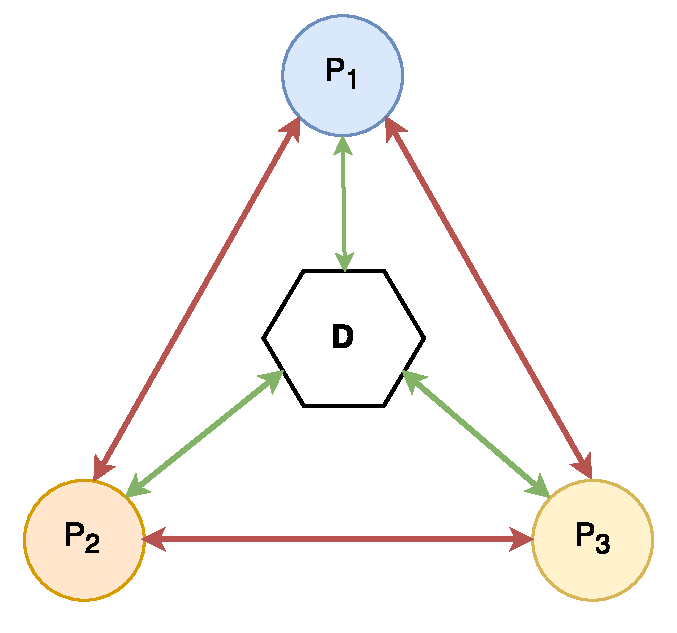
\includegraphics[width=0.5\textwidth]{imagenes/architecture.pdf}
  \caption{Conexión entre nodos \texttt{Directorio} y Participantes}
  \label{fig:connections-directory-participants}
\end{figure}

La funcionalidad de proveer un punto de entrada a la sala también se podría 
realizar entre los propios nodos \texttt{Participantes}, sin la necesidad de 
incorporar un nodo \texttt{Directorio}. Si bien en esta investigación se 
priorizó la facilidad de implementar la variante utilizando el nodo adicional, 
se podría ejecutar alguna variante de \emph{gossip protocol} 
\cite{Demers:1987:EAR:41840.41841} para informar la identidad de participantes 
nuevos que vayan entrando a la sala, lo cual podría solucionar el problema. 
Esta segunda variante además tiene la ventaja de no poseer un punto vulnerable 
(que sería el nodo \texttt{Directorio}), evitando ataques directos al nodo 
\texttt{Directorio}, retrasando (o incluso imposibilitando) la 
creación del \emph{anonymity set}. 
<<MEJORAR LA SIGUIENTE FRASE:>>Reiterar que se implementó el nodo 
\texttt{Directorio} por simplicidad, pero se tienen en cuenta los posibles 
ataques que puede recibir el sistema, que no tienen incidencia en romper el 
anonimato que brinda el protocolo.

Actualmente el nodo \texttt{Directorio} inicia estableciendo los 
parámetros públicos del protocolo y publica su dirección IP. Luego, cada nodo 
Participante que se quiera unir se conecta a la dirección pública del 
\texttt{Directorio} y espera que se complete la cuota de participantes 
establecida en un comienzo. Cuando se conectan los $n$ participantes 
necesarios, el \texttt{Directorio} informa la dirección IP de cada uno de los 
participantes a todo el resto, para que posteriormente inicien el protocolo 
solo enviándose mensajes entre ellos. Esto termina la labor del nodo 
\texttt{Directorio}. En la Figura \ref{fig:connections-directory-participants} 
se observa las conexiones que se realizan durante el desarrollo del protocolo, 
primero conectando cada participante que viene entrando a la sala al nodo 
\texttt{Directorio} (representado por las conexiones verdes), y luego que 
todos los participantes se hayan conectado al nodo \texttt{Directorio}, éste 
le comunica a toda la sala las direcciones de los nodos \texttt{Participantes} 
presentes, terminando su labor, desconectándose de los nodos 
\texttt{Participantes}, y estos finalmente se conectan mediante los enlaces 
rojos entre cada uno de ellos. En la Figura \ref{fig:connections-participants} 
se observa en mayor detalle la conexión entre cada par de participantes, la 
cual se realiza a través de \emph{sockets} tipo \emph{requestor-replier}, 
formando así el \emph{anonymity set} deseado, y continuando con el normal 
desarrollo del protocolo anteriormente descrito.

\begin{figure}[H]
  \centering
    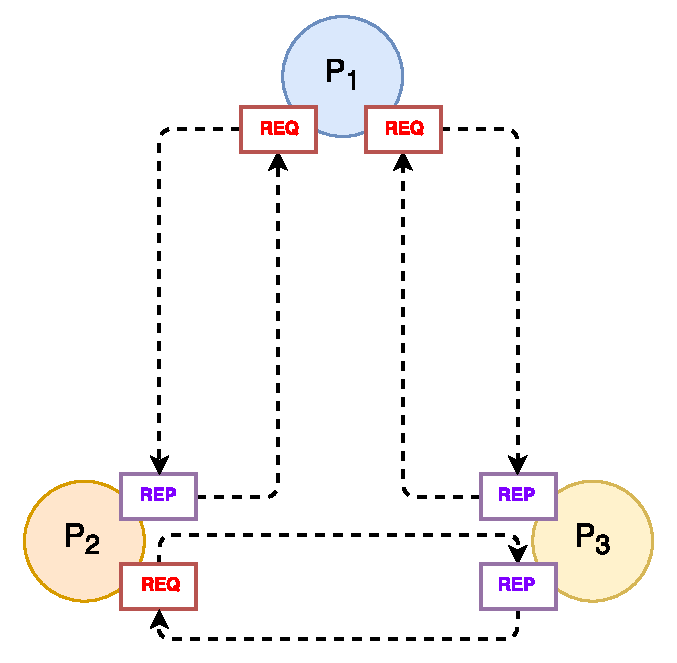
\includegraphics[width=0.5\textwidth]{imagenes/participants_connection.pdf}
  \caption{Conexión entre nodos \texttt{Participantes}}
  \label{fig:connections-participants}
\end{figure}

\section{Primitivas Criptográficas}

En la implementación actual, la gran mayoría de las primitivas criptográficas 
han sido implementadas desde cero, valiéndose principalmente de la biblioteca 
para manejar números grandes de \emph{Java}, \emph{BigInteger}\footnote{\url{
https://docs.oracle.com/javase/7/docs/api/java/math/BigInteger.html}}. Si bien 
esto no es una práctica recomendada (lo ideal es utilizar bibliotecas 
criptográficas ya probadas por la comunidad), se decidió por esto luego de no 
encontrar bibliotecas que implementaran las funcionalidades requeridas por el 
protocolo (\emph{Pedersen Commitments} y \emph{ZKP} asociadas). Como fue 
dicho, la implementación de primitivas criptográficas no es recomendado. Más 
bien, se recomienda utilizar implementaciones ya probadas y verificadas por la 
comunidad, como lo podría ser 
Charm-Crypto\footnote{\url{http://charm-crypto.com/index.html}} o 
Scapi\footnote{\url{https://scapi.readthedocs.io/en/latest/}}. De todas 
maneras, la criptografía implementada se desarrolló utilizando interfaces, por 
lo que de tener una librería que cumpla los requerimientos criptográficos 
indicados en el Capítulo 3, su implantación podrá ser realizada de manera 
expedita y transparente al resto de la implementación.

\section{\emph{API} implementada}

Como fue dicho anteriormente, una contribución importante de este trabajo 
es implementar una \emph{API} disponible para toda la comunidad. Esta API 
permitirá a la comunidad una aplicación que esté basada en el protocolo 
anteriormente descrito. 

La implementación anterior fue empaquetada como librería \emph{Java}, 
utilizable por otras aplicaciones al importar el archivo \emph{.jar} generado. 
Esta librería quedó con los siguientes métodos de manera pública, formando así 
la \emph{API} disponible:

\begin{itemize}
    \item \texttt{DCNETProtocol class:} clase base que entrega la \emph{API} 
    que es necesario instanciar para utilizar los métodos descritos a 
    continuación. 
    \item \texttt{boolean connectToDirectory():} luego de setear la dirección 
    IP del nodo \texttt{Directorio}, este método realiza la conexión desde el 
    nodo \texttt{Participante} hacia el \texttt{Directorio}, utilizando las 
    funciones provistas por la librería \emph{ZeroMQ}.
    \item \texttt{void setMessageToSend(String s, boolean b):} este método 
    tiene como finalidad permitir al nodo \texttt{Participante} establecer el 
    mensaje que desea comunicar al resto de la sala utilizando el protocolo. 
    \item \texttt{void runProtocol(PrintStream p):} corre el protocolo 
    anteriormente descrito de manera automática, calculando los diferentes 
    \emph{commitments} y \emph{zero-knowledge proofs} necesarios, repitiendo 
    las rondas necesarias y finalizando cuando todos los mensajes han sido 
    recibidos por la totalidad de los participantes en cuestión.
    \item \texttt{ObservableParticipantsLeft:} objeto que emplea el patrón de 
    diseño \emph{Observer} para ir informando cuáles participantes se van 
    conectando a la sala a medida que va ocurriendo, y así tener una noción de 
    cuantos participantes faltan para completar la cuota puesta en un 
    principio por el nodo \texttt{Directorio}.
    \item \texttt{ObservableMessagesArrived:} también emplea el patrón de 
    diseño \emph{Observer} para informar al participante de los mensajes que 
    van resultando de correr el protocolo, a medida que éste avanza. 
    Importante señalar que los mensajes se despliegan en tiempo real.
\end{itemize}

\section{Aplicación Móvil}

Para poder probar el uso de la \emph{API} implementada, se desarrolló una 
aplicación móvil prototipo, que tiene como objetivo permitir un uso 
simplificado 
del protocolo implementado, que permita a los usuarios montar una conversación 
que asegure el anonimato de sus participantes.

La aplicación está compuesta de 3 módulos: (1) conexión al nodo 
\texttt{Directorio}, (2) envío del mensaje por parte del participante, y (3) 
recepción de los mensajes del resto de los participantes de la sala.

\begin{figure}[H]
    \centering
    \begin{subfigure}[b]{0.4\textwidth}
        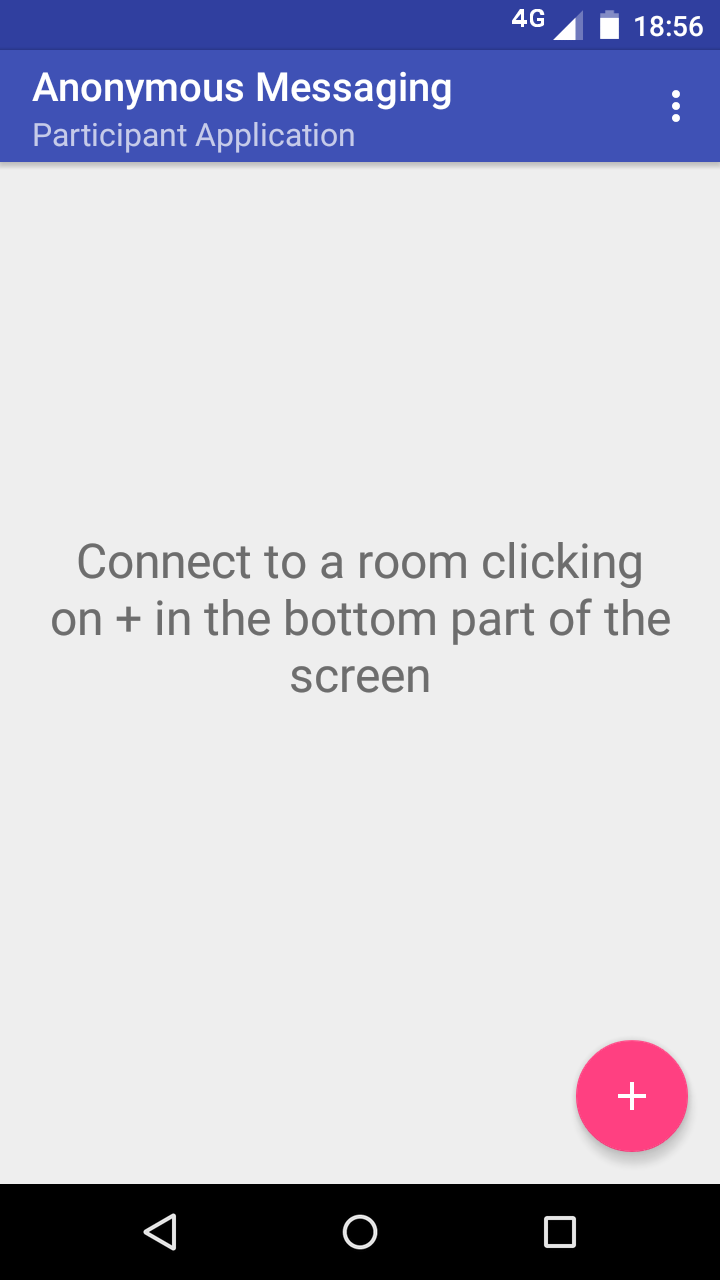
\includegraphics[width=\textwidth]{imagenes/mobile_first.png}
        \caption{Conexión al Nodo \texttt{Directorio}}
        \label{fig:mobile_connect}
    \end{subfigure}
    ~
    \begin{subfigure}[b]{0.4\textwidth}
        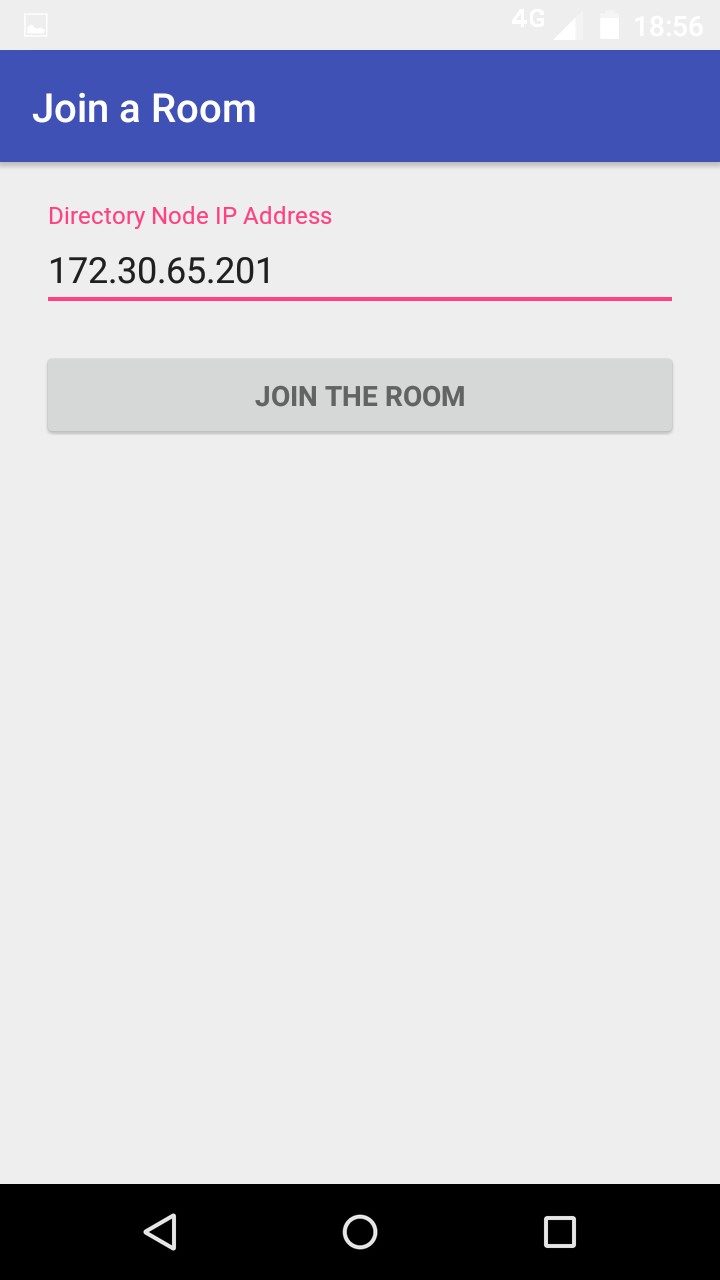
\includegraphics[width=\textwidth]{imagenes/mobile_connect.png}
        \caption{Establecer dirección del \texttt{Directorio}}
        \label{fig:mobile_set_ip}
    \end{subfigure}
    \caption{Screenshots de Aplicación Móvil (parte 1)}
    \label{fig:mobile_screenshots_1}
\end{figure}

\begin{figure}[H]
    \centering
    \begin{subfigure}[b]{0.4\textwidth}
        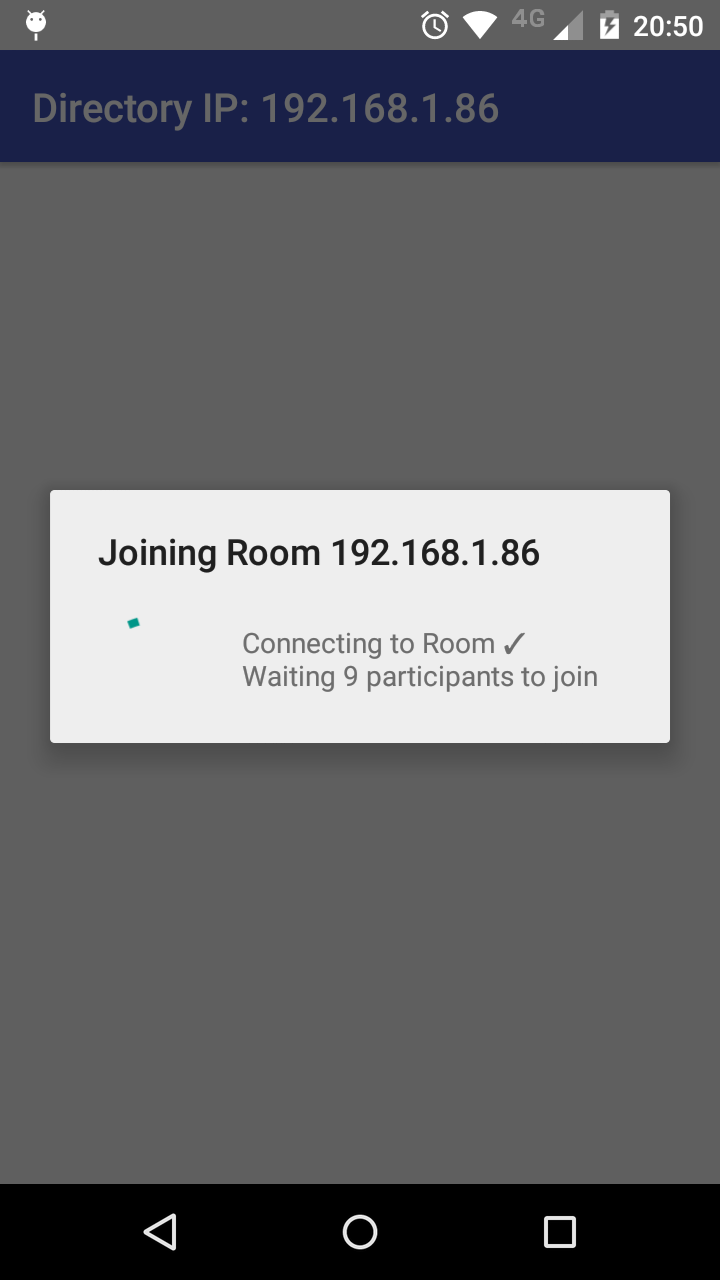
\includegraphics[width=\textwidth]{imagenes/mobile_connecting.png}
        \caption{Esperando conexión a Sala}
        \label{fig:mobile_waiting}
    \end{subfigure}
    ~
    \begin{subfigure}[b]{0.4\textwidth}
        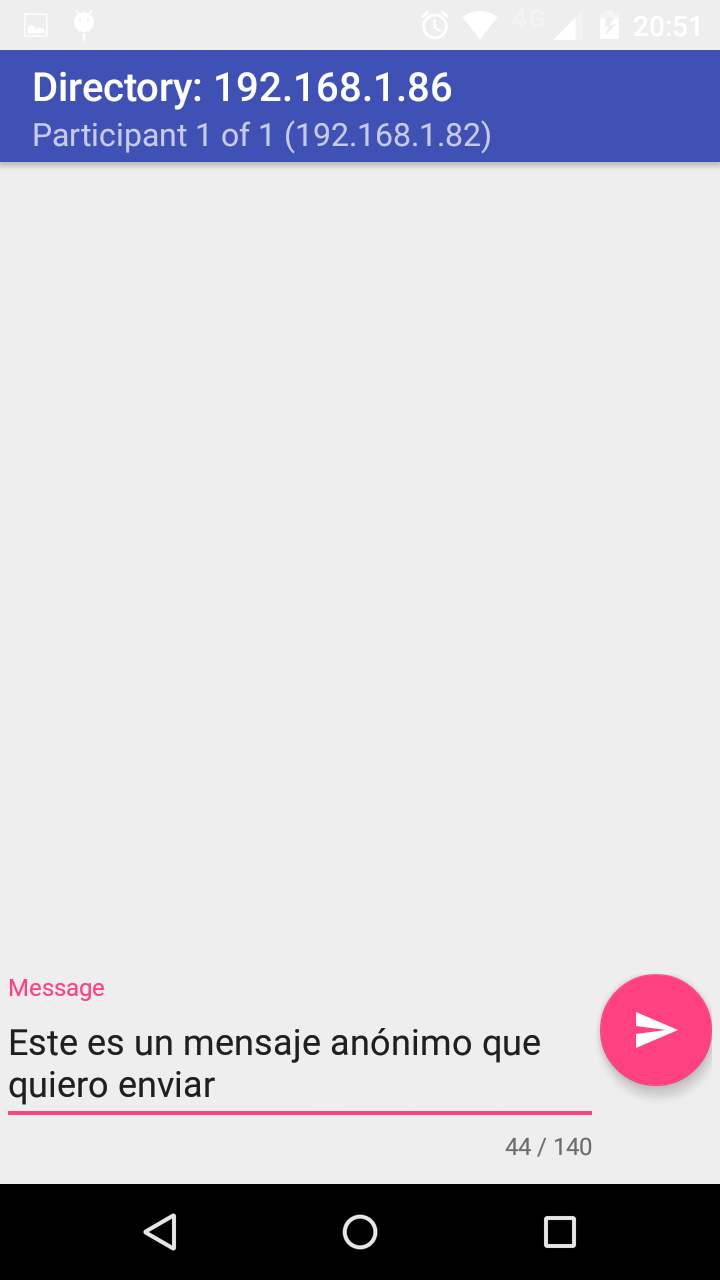
\includegraphics[width=\textwidth]{imagenes/mobile_message.png}
        \caption{Envío del mensaje a la sala}
        \label{fig:mobile_set_msg}
    \end{subfigure}
    \caption{Screenshots de Aplicación Móvil (parte 2)}
    \label{fig:mobile_screenshots_2}
\end{figure}

\chapter{Experimentación y Resultados}
\section{Infraestructura utilizada}

\subsection{Simulación de Red}



\subsection{Uso de red real}




\section{Resultados}
\chapter{Trabajo Futuro}

Entre más se avanzaba en el trabajo desarrollado, mayor era la posibilidad de transformar
una investigación académica-científica en una herramienta disponible para múltiples
usuarios en el mundo que deseen transmitir información de manera anónima y simple, 
utilizando su dispositivo móvil.

Para lograr dicho objetivo aun falta trabajo que realizar, sobre todo en la capa de
comunicación entre los distintos nodos partícipes del protocolo. Las tareas que se
realizarán a futuro son las siguientes:

\begin{enumerate}
    \item Autenticar canales: la seguridad del protocolo criptográfico se basa fuertemente
    en que los canales de comunicación que existan entre los distintos nodos participantes
    sean autenticados, es decir, que cada usuario debe enviar sus mensajes firmados, para
    así el receptor de cada mensaje se asegure que el emisor es quien dice ser. Con esto
    se evitan participantes impostores, es decir, que se hagan pasar por otro 
    participante, lo que podría resultar en bajar la reputación de algún usuario,
    eliminándolo de la sala.
    
    \item Manejar desconexión de usuarios: cualquier aplicación que pretenda ser utilizada
    en ambientes ``reales'' debe manejar la posible desconexión de usuarios en cualquier 
    momento del protocolo. Actualmente esto no es manejado y simplemente la aplicación 
    deja de funcionar. Es importante además, que cualquier medida que se adopte, se 
    verifique que no influye en el anonimato y seguridad de los participantes. Por 
    ejemplo se puede adoptar la medida de ``simular'' al participante desconectado 
    suponiendo que envía mensajes vacíos, pero hay que establecer si esta medida no 
    afecta tanto la integridad del protocolo (los mensajes que aun no se reciben 
    se van a enviar satisfactoriamente) como el anonimato y seguridad de los 
    participantes que quedan involucrados, o incluso el mismo participante que sufrió 
    la desconexión (se podría saber que el participante que se desconectó envió o no 
    envió alguno de los mensajes publicados anteriormente).
    
    \item Manejar participantes maliciosos: actualmente el protocolo y la implementación 
    es capaz de encontrar a un participante malicioso, pero más allá de identificarlo 
    no emplea ninguna medida en contra de éste. Podría seguir el protocolo suponiendo 
    la desconexión del participante malicioso, lo que sería análogo al punto anterior, 
    pero tal vez existan medidas más drásticas como suspensión por un cierto tiempo 
    de participar en otras sesiones del protocolo, o derechamente la expulsión del 
    participante para siempre. 
    
    \item Optimizar recepción de mensajes: una parte importante a analizar por gente 
    más experta en el área de Redes es la manera en que se están recibiendo los 
    mensajes por parte de los participantes. Actualmente se delegó toda responsabilidad 
    a \emph{ZeroMQ}, el cual emplea una cola para no perder los mensajes entrantes 
    y la implementación actual se queda esperando entre mensajes, sin realizar 
    ninguna operación. Tal vez sea necesario revisar ese protocolo y optimizar la recepción de mensajes, abriendo múltiples \emph{sockets}, o utilizando el tiempo de espera entre mensajes para poder realizar alguna operación criptográfica pendiente, 
    y así no tener tiempo ocioso.
    
    \item Refinar protocolo criptográfico: 
    
    \item Mejorar diseño de aplicación móvil:
    
    \item Utilizar aplicación a través de Internet:
    
    \item Pruebas de seguridad:
\end{enumerate}
\chapter{Conclusión}

\todo{completar esto}

% \input{glosario.tex} % opcional

\bibliographystyle{plain}
\bibliography{bibliografia}

% \chapter{Apéndice}

\section{Apéndice A: Descripción de \emph{Zero-Knowledge Proofs}}\label{apen-a}

\subsection{Consideraciones Generales}

Las \emph{Zero-Knowledge Proofs} necesitadas para el desarrollo de este 
trabajo son del tipo \emph{proof-of-knowledge}, las cuales permiten a un 
participante, el \emph{prover}, demostrarle a otro participante, el \emph{verifier}, que conoce un cierto 
valor (o varios valores) que hacen verdadera una cierta proposición, sin la 
necesidad de revelar dicho valor. Por ejemplo, a través de esta técnica 
criptográfica una persona podría demostrar que conoce todos los 
valores que solucionan un cierto tablero de \emph{sudoku}, sin la necesidad de 
revelar estos valores.

Generalmente estas demostraciones son \emph{interactivas}, es decir, 
\emph{prover} y \emph{verifier} se comparten distintos valores durante el 
desarrollo del protocolo, lo cual finalmente convence al \emph{verifier} de la 
propiedad que se quería demostrar. Eso si, casi toda demostración interactiva puede 
transformarse a \emph{no interactiva}, es decir, sin la necesidad de 
intercambiar valores. El \emph{prover} puede demostrar el conocimiento de 
cierto valor solamente a través del cálculo de algunos valores, suponiendo que 
existen otros valores que son públicamente conocidos (en particular, conocidos 
por el \emph{verifier}). Las demostraciones utilizadas en este trabajo y 
detalladas a continuación son no interactivas.

\subsection{Logaritmo Discreto}

$$PoK\{w: y = g^w\}$$

Sean $g, y$ valores públicos, tales que $g$ es generador de un grupo cíclico $G$ de orden primo $q$, y 
$y \in G$. 
El \emph{prover} (de identidad pública 
\texttt{id}) debe demostrar que conoce el valor $w$ que hace verdadera la 
siguiente proposición: $y = g^w$. Los pasos que debe seguir son los siguientes:
\begin{enumerate}
	\item Escoger $r \in \mathbb{Z}_q$ aleatorio.
	\item Calcular $z = g^r$
	\item Calcular $b = H(z \mid\mid g \mid\mid y \mid\mid \mathtt{id})$, 
	donde $H(\cdot)$ es una función de hash resistente a colisiones (por ejemplo, 
	\texttt{SHA3}), tal que $H: \sum^{n} \rightarrow \mathbb{Z}_q$.
	\item Calcular $a = r + bw \pmod q$
	\item Enviar como demostración la tupla $\mathcal{D} = (g, z, a)$
\end{enumerate}

Finalmente, el \emph{verifier} debe recibir la demostración $\mathcal{D}$ y 
verificarla siguiendo estos pasos:
\begin{enumerate}
	\item Calcular $\hat{b} = H(z \mid\mid g \mid\mid y \mid\mid \mathtt{id})$ 
	utilizando la misma función de hash usada por el \emph{prover}.
	\item Verificar que $g^a = y^{\hat{b}} z$
\end{enumerate} 

Este protocolo también es conocido como \emph{Firma de Schnorr} y para más detalles 
sobre su seguridad y correctitud revisar \cite{schnorr1989efficient}.

\subsection{Uno de dos logaritmos discretos}

$$PoK\{x_1, x_2 : h_1 = g^{x_1} \lor h_2 = g^{x_2}\}$$

Sean $g,h_1,h_2$ valores públicos. El \emph{prover} (de identidad pública 
\texttt{id}) debe demostrar que conoce al menos uno de los valores $(x_1,x_2)$ 
que hacen verdad la siguiente proposición: $h_1 = g^{x_1} \lor h_2 = g^{x_2}$. 
Los pasos que debe seguir son los siguientes (sin pérdida de generalidad, 
supondremos que conoce el valor $x_1$):
\begin{enumerate}
	\item Escoger $c, r_1, r_2$ aleatorios.
	\item Calcular $z_1 = g^{r_1}$
	\item Calcular $z_2 = g^{r_2} h_2^{-c}$
	\item Calcular $b = H(z_1 \mid\mid z_2 \mid\mid g \mid\mid h_1 \mid\mid h_2 \mid\mid \mathtt{id})$, donde $H(\cdot)$ es una función de hash resistente a colisiones (por ejemplo, \texttt{SHA3}).
	\item Calcular $t = b - c$
	\item Calcular $a = r_1 + t x_1$
	\item Enviar como demostración la tupla $\mathcal{D} = (t, c, z_1, z_2, a, r_2)$.
\end{enumerate}

Finalmente, el \emph{verifier} debe recibir la demostración $\mathcal{D}$ y 
verificarla siguiendo estos pasos:
\begin{enumerate}
	\item Calcular $\hat{b} = H(z_1 \mid\mid z_2 \mid\mid g \mid\mid h_1 \mid\mid h_2 \mid\mid \mathtt{id})$ utilizando la misma función de hash usada por el \emph{prover}.
	\item Verificar que $\hat{b} = t + c$
	\item Verificar que $g^a = h_1^t z_1$
	\item Verificar que $g^{r_2} = h_2^c z_2$
\end{enumerate} 

El protocolo descrito anteriormente es un caso específico del esquema propuesto en \cite{cramer1994proofs}, en el cual se describe la manera de demostrar el conocimiento de un subconjunto de valores dentro de un cierto \emph{statement} (en el caso necesario para este trabajo, se demostró el conocimiento de sólo un valor de dos posibles). 

\subsection{Dos logaritmos discretos}

$$PoK\{x_1, x_2 : h_1 = g^{x_1} \land h_2 = g^{x_2}\}$$

Sean $g,h_1,h_2$ valores públicos. El \emph{prover} (de identidad pública 
\texttt{id}) debe demostrar que conoce ambos valores $(x_1,x_2)$ que hacen 
verdad la siguiente proposición: $h_1 = g^{x_1} \land h_2 = g^{x_2}$. Los 
pasos que debe seguir son los siguientes:
\begin{enumerate}
	\item Escoger $r_1, r_2$ aleatorios.
	\item Calcular $z_1 = g^{r_1} $
	\item Calcular $z_2 = g^{r_2}$
	\item Calcular $b = H(z_1 \mid\mid z_2 \mid\mid g \mid\mid h_1 \mid\mid h_2 \mid\mid \mathttt{id})$, donde $H(\cdot)$ es una función de hash resistente a colisiones (por ejemplo, \texttt{SHA3}).
	\item Calcular $a_1 = r_1 + b x_1$
	\item Calcular $a_2 = r_2 + b x_2$
	\item Enviar como demostración la tupla $\mathcal{D} = (z_1, z_2, a_1, a_2)$.
\end{enumerate}

Finalmente, el \emph{verifier} debe recibir la demostración $\mathcal{D}$ y verificarla siguiendo estos pasos:
\begin{enumerate}
	\item Calcular $\hat{b} = H(z_1 \mid\mid z_2, \mid\mid g \mid\mid h_1 \mid\mid h_2 \mid\mid \mathtt{id})$ utilizando la misma función de hash usada por el \emph{prover}.
	\item Verificar que $g^{a_1} = z_1 h_1^\hat{b}$
	\item Verificar que $g^{a_2} = z_2 h_2^\hat{b}$
\end{enumerate}

El protocolo anterior resulta de realizar en paralelo dos demostraciones como la descrita en \cite{schnorr1989efficient} (conocimiento de logaritmo discreto).

\subsection{Valores en \emph{Pedersen Commitments}}

$$PoK\{x, r : c = g^x h^r\}$$

Sean $c, g, h$ valores públicos. El \emph{prover} (de identidad pública 
\texttt{id}) debe demostrar que conoce ambos valores $(x,r)$ que hacen verdad 
la siguiente proposición: $c = g^x h^r$. Los pasos que debe seguir son los 
siguientes:
\begin{enumerate}
	\item Escoger $y, s$ aleatorios.
	\item Calcular $d = g^y h^s$
	\item Calcular $e = H(d \mid\mid g \mid\mid h \mid\mid c \mid\mid \mathtt{id})$, donde $H(\cdot)$ es una función de hash resistente a colisiones (por ejemplo, \texttt{SHA3}).
	\item Calcular $u = ex + y$
	\item Calcular $v = er + s$
	\item Enviar como demostración la tupla $\mathcal{D} = (d, u, v)$.
\end{enumerate}

Finalmente, el \emph{verifier} debe recibir la demostración $\mathcal{D}$ y 
verificarla siguiendo estos pasos:
\begin{enumerate}
	\item Calcular $\hat{e} = H(d \mid\mid g \mid\mid h \mid\mid c \mid\mid \mathttt{id})$ utilizando la misma función de hash usada por el \emph{prover}.
	\item Verificar que $g^u h^v = c^\hat{e} d$
\end{enumerate}
 % opcionales

\end{document}
